% !TEX root=frame_thesis.tex
\chapter{Methods and Model Description}\label{chapter:Methods}

\section{Overview of the Model}
%Topic: General overview of ABM
%Main Idea: Human agents interact with local Environment
I present an Agent-Based Model (ABM) that simulates the pre-historic temporal and spatial pattens of household agents on Easter Island and their interactions with the natural environment. 
The environment is encoded on a 2D discretised map with heterogeneous, geographic features.
Agents rely both on a limited, non- or slowly renewable resource, the palm trees, and a limited, renewable resource, the arable land (in particular used for sweet potato cultivation). 
They obtain these resources by cutting trees and farming viable sites in their near surroundings, thereby changing their local environment.
Consequently, the household's population growth or decline depends on the success of this resource acquisition. 
Furthermore, resource availability and other geographic indicators determine the settlement behaviour of the agents.
The interaction with the natural environment, thus, constrains the settlement patterns as well as the population dynamics of the overall Easter Island society.

%Topic: Time and Update Order
The model assumes yearly updates of the characteristic variables of each household agent and the environment throughout the simulated time period.
The simulation starts with the arrival of the first settlers at Anakena Beach in
\begin{equation}
t_\text{arrival} = 800\, {\rm A.D.}\ .
\end{equation}
The initial population is assumed to be $\mathbf{pop}_{\rm arrival} = 40$ individuals (as in \citet{Good2006}, \citet{Brander1998}, and similar to \citet{Brandt2015}) spread on $2$ households, that both settle close to Anakena Beach.
Each time step, $\Delta t=1\,{\rm yr}$, all agents are updated and interact with their local environment sequentially in a randomised order. 
New household agents can appear throughout the simulation following reproduction and splitting of existing agents. 
Following the alteration of the environment by all agents, the environment's state variables are updated once per year, denoted as natural update here (e.g.\ potential regeneration, or soil degradation).
The simulation ends in $1800\, {\rm A.D.}$ with the arrival of European voyages marking the end of the isolated status of the pre-historic Easter Island society.%, since this presumably had a large impact on the society, e.g.\ through the introduction of diseases wiping out a large fraction of the Easter Island population in the 19th century.% \todo{cite Bahn2017}.

%Topic: I will describe the Model
In Section \ref{sec:CreateMap}, I describe the generation of the 2D discretised map comprising the environment of Easter Island as well as the yearly natural updates. In Section \ref{sec:AgentUpdate}, I then focus on the household agents and the update procedure of a single agent:
%This update is separated into several modules: Calculating of the agents' resource requirements, cutting trees, farming, increasing/decreasing population of the agent, and potentially moving the settlement.
A single update comprises an adjustment of the agent specific properties, described in Section \ref{sec:AgentUpdate}, the interaction between an agent and the environment, described in Section \ref{sec:Harvest}, and the consequent response of the agent's properties to the harvest, i.e.\ population growth or decline and potential re-settlement, described in Section \ref{sec:Reaction}.
Figure \ref{fig:SketchABM} summarises all environmental variables, the agent variables, and their dependencies (except for re-settlement, which is described later in Figure \ref{fig:sketchmoving}).

\begin{figure}[H]
	\centering
	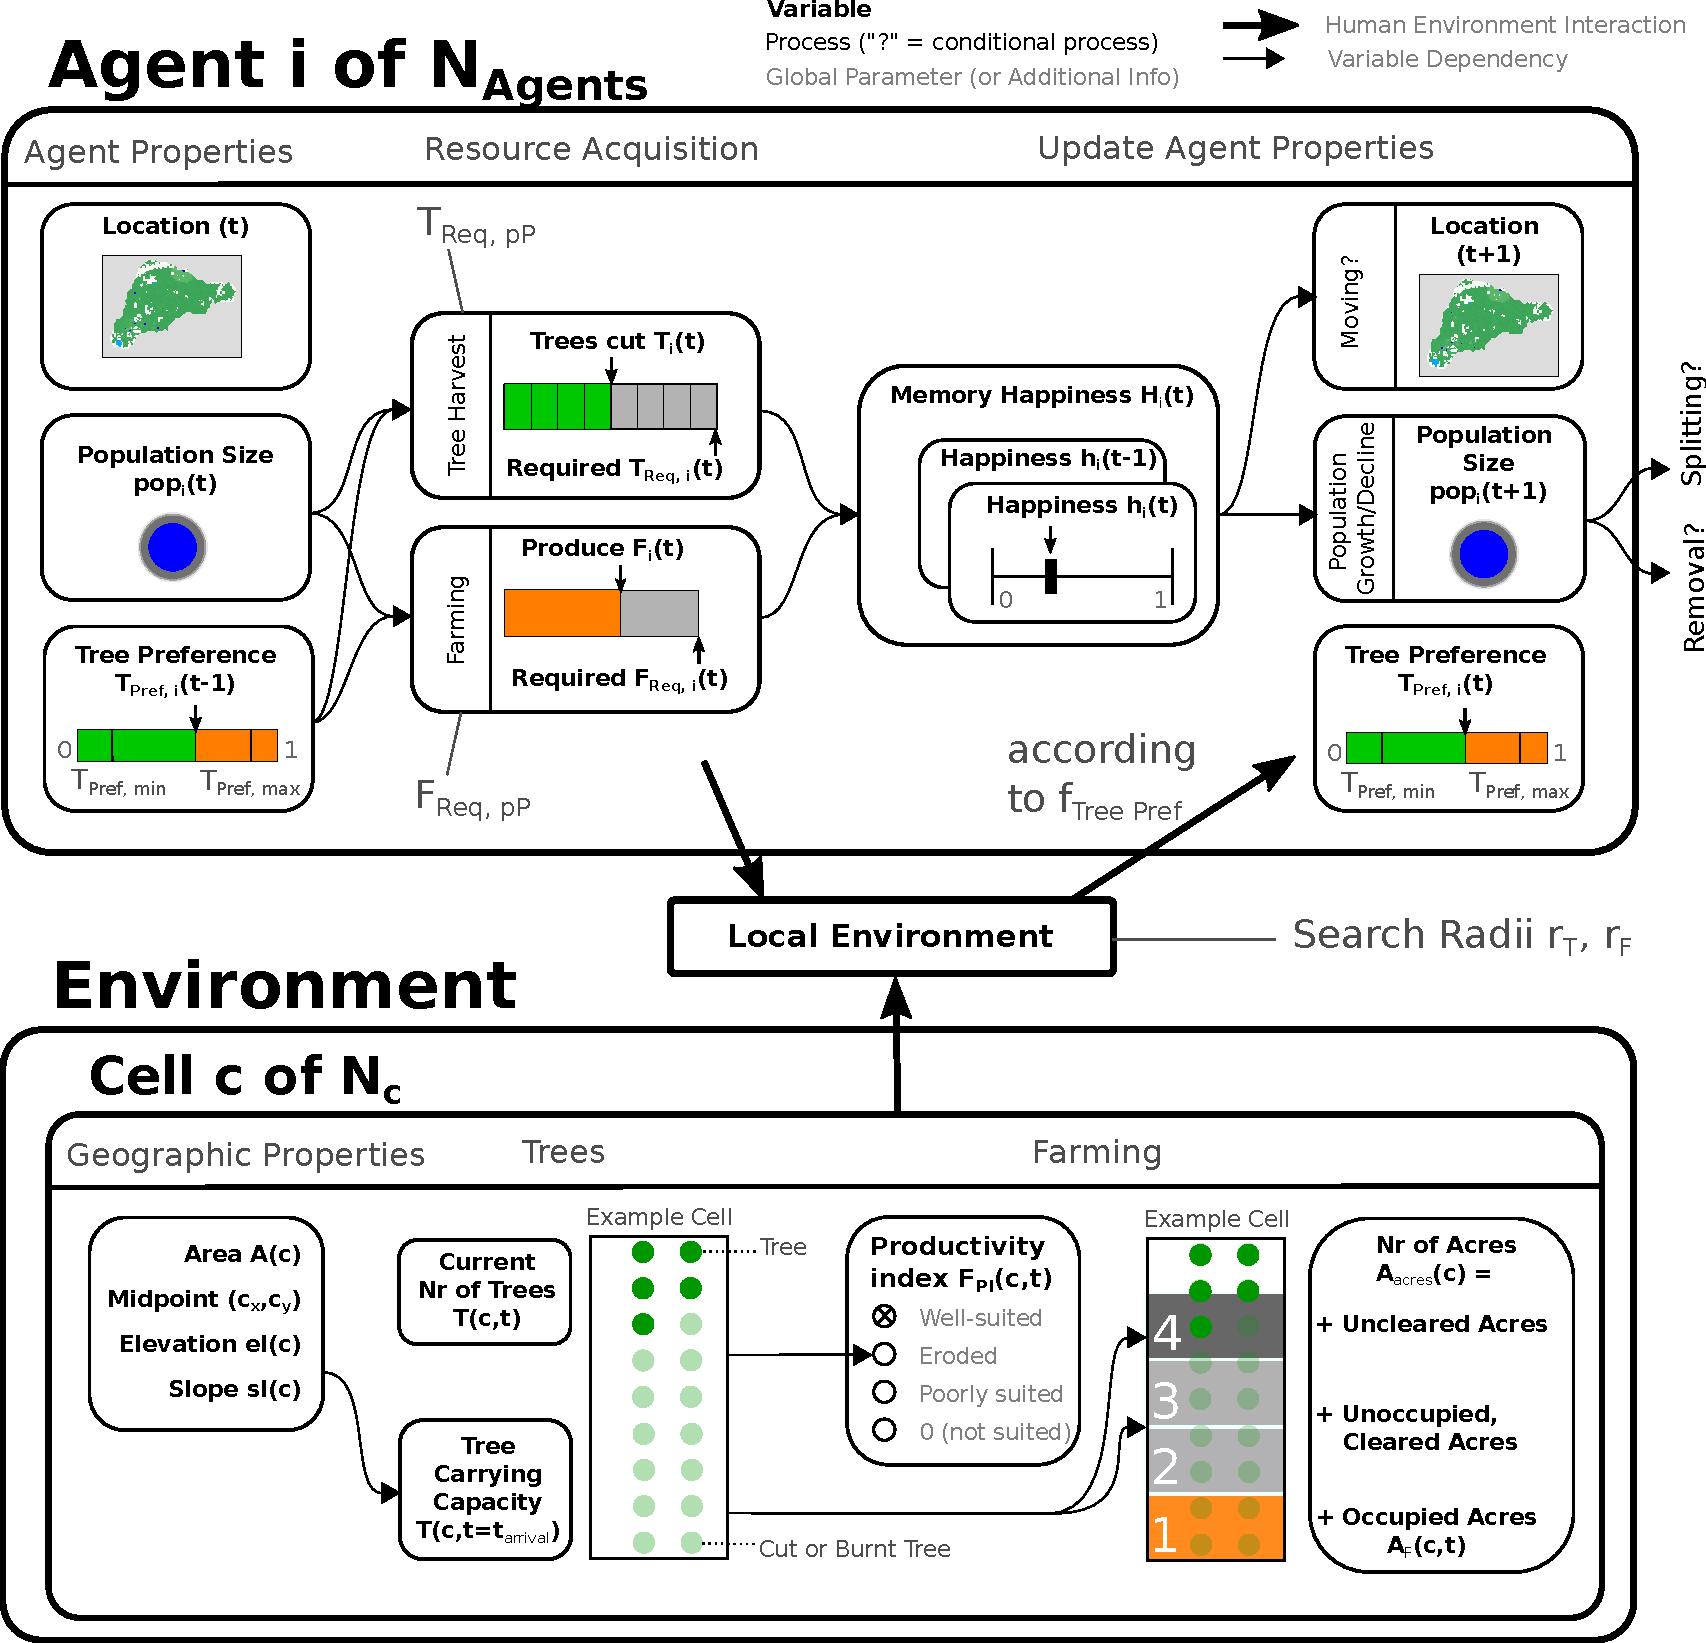
\includegraphics[width=1\textwidth]{images/SketchABM2/sketch.pdf}
	\caption{
		A sketch of an update step of agent $i$ in this ABM, which is described in detail in Chapter \ref{chapter:Methods}.
		The environment consists of $N_\text{c}$ discretised cells, $c$, with certain geographic properties: Area $A(c)$, midpoint $\vec{c}$, terrain elevation $el(c)$, and slope $sl(c)$.  %population density $\frac{pop(C_\text{F}(t)}{r_\text{F}^2\pi}$) (within cells in a circle with radius $r_{\rm F}$, $C_{\rm F}(c)$) 
		A cell has furthermore two `resource stocks'.
		The first resource stock is the number of trees $T(c,t)$, with a maximum of the cell's carrying capacity (and initial state) $T(c,t=t_{\rm arrival})$, which depends on $el(c)$ and $sl(c)$. 
		The second resource stock is the number of arable (i.e.\ cells with a Farming Productivity Index $F_{\rm PI}(c,t)>0$) sites, $A_\text{acres}(c)$, with a basic unit of $1\, {\rm acre}$, consisting of uncleared, cleared but unoccupied and occupied sites ($\mathbf{A}_\text{F}(c,t)$ in acres).
		Agent $i$ represents a household with a population size $pop_\text{i}(t)$, a settlement location $(x_\text{i},\, y_\text{i})(t)$ (corresponding cell $c_\text{i}(t)$), and a tree preference $T_\text{Pref, \, i}(t-1)$, reflecting the state of the local environment in the previous year. From the population size and tree preference (and global, tunable per person resource requirement parameters, $T_{requ, \, pP}$ and  $F_\text{requ, \, pP}$) the corresponding requirements for tree cutting, $T_\text{Req, \, i}(t)$ and farming, $F_\text{Req, \, i}(t)$, are calculated each year.
		The success of the resource acquisition from the local environment determines the current and memory happiness of the agent, $h_{\rm i}(t)$ and $H_{\rm i}(t)$. %requirements depends on the resource stocks of cells in radii $r_{\rm T}$ for tree harvest and $r_{\rm F}$ for farming. 
		This latter then determines the agent's population dynamics (including potential splitting or dispersion of the agent) and whether or not the agent relocates the settlement (according to a semi-rationale decision making process sketched in Figure \ref{fig:sketchmoving} later).
		Finally, the tree preference, $T_\text{Pref, i}(t)$ is updated reflecting the state of the changed local environment.
	}
	\label{fig:SketchABM}
\end{figure}


\section{Creating a 2D discretised Map of Easter Island}\label{sec:CreateMap}
I create a discretised map dividing the island into a number of small 2D triangular cells with certain geographical features.
I use a 2D equidistant grid ranging $18\, {\rm km}$ in latitudinal (from $-27.2050^\circ N$ to $-27.0437^\circ N$) and $24\, {\rm km}$ in longitudinal direction (from  $-109.4650^\circ E$ to 
 $-109.2227^\circ E$).
The grid size is  $\delta_{\rm x} \approx 320\, {\rm m}$ between points in $x$- (i.e.\ $75$ points) and $\delta_{\rm y} \approx 360\, {\rm m}$ between points in y-direction (i.e.\ $50$ points). 
In principle, the map can be created with any arbitrary resolution, constrained only by the resolution of the underlying geographical data. 
Also other grid types, e.g.\ with adaptive grid lengths to focus on regions of interest, are completely compatible with the model. 
While a higher resolution increases detailed geographical representation and reduces discretisation errors, computation time of the presented model scales highly non-linearly (see Section \ref{sec:Reaction}).
Hence, a trade-off has to be found between detail or accuracy and computation time.
I create 2D triangular cells from this grid using \citet{matplotlib}'s Delaunay triangulation package.
A cell $c$ is characterised by its midpoint $\vec{c} = (c_{\rm x},\, c_{\rm y})$. 
Since all cells are Delaunay triangles, their smallest angles are maximised and, hence, the midpoint, $\vec{c}$, provides a reasonable representation of the cell.
%Topic: Define Easter Island
%Using geographical information, the triangles making up Easter Island are selected.
The terrain features, elevation, $el(c)$, and slope, $sl(c)$, of Easter Island are obtained from a publicly available, high resolution elevation map \citep{Jarvis2008CIGAR} via Google Earth Engine \citep{gorelick2017google} and evaluated at the corresponding midpoint $\vec{c}$.
All cells located on the ocean (i.e.\ $c$ with $el(c)=0$) are masked out and discarded.
The cells corresponding to the island's three small crater lakes (in some periods reduced to two due to drought periods) are also identified.
The remaining cells constitute the landmass of the discretised island, which can later be settled, deforested or farmed by the agents. 
With the resolution given above, $N_{\rm c} = 2768$ cells remain with an area of roughly $A(c)= 0.06 \, {\rm km^2} = 14.2 \, {\rm acre}$.
The area of the discretised Easter Island is $A=159.2\, {\rm km^2}$, ($163.6\, {\rm km^2}$ in reality) providing a detailed, cellular representation of geographical features (location $\vec{c}$, area $A(c)$, elevation $el(c)$, and slope $sl(c)$).

%There are three -- or two in periods of major droughts (see \citet{Rull2020}) -- permanent crater lakes on Easter Island, providing the major freshwater sources for the prehistoric Easter Island population, as discussed later in Section \ref{sec:Moving}.
%The corresponding cells are calculated from the locations and radii of these lakes. 
%This procedure gives a detailed, discretised representation via triangular cells with geographical features of Easter Island. 
 
%Archaeological records indicate that crater lakes could have dried out during major drought periods.
%In particular the drying of Rano Raraku in the East of Easter Island during the Medieval Climate Anomaly ($500-1200 \, \rm{A.D.}$) and during the Little Ice Age ($1570-1720\, \rm{A.D.}$) \citep{Rull2020} and the consequences have been a reoccuring theme of scientific debate (e.g.\ \citet{Cauwe2011}). 
%Such drought events can be simulated by removing each of the lakes for some period of time from the map.

Next to the geographical features described above, a cell has characteristic biological features.% next to the geographic specification before. 
Each cell $c$ has a tree number, denoted as $T(c,t)$ (or tree density $T(c,t)/A(c)$).
While the assumption of constant climatic conditions throughout Easter Island's history has been challenged recently \citep{Rull2020}, I only consider anthropogenic deforestation $T(c,t)$.
Hence, the island's forest system is assumed to be in equilibrium (c.f.\ \citet{Brander1998}) at the time of the arrival of the first settlers, $t_\text{arrival}$ and, thus, $T(c,t=t_\text{arrival})$ is the constant carrying capacity of palm trees for each cell $c$ on the island. 
There is is still some uncertainty about the total number and spatial patterns of palm trees at $t=t_\text{arrival}$.
\citet{Mieth2015} estimate a total of $16\cdot 10^6$ trees covering $80\%$ of the island from root casts in the soil, whereas e.g.\ \citet{Brandt2015} initialise the model with a conservative estimate of $8\cdot 10^6$ trees. 
Most studies assume an island wide, dense distribution of the palm trees. 
E.g.\ \citet{Bahn2017} state that soil sufficient for tree growth is present `almost everywhere on the island, apart from the steepest parts of the cliffs and the youngest lava surfaces' (i.e.\ the highest elevations of Mount Terevaka). 
However, \citet{Rull2020} also investigates the possibility of mosaic vegetation patterns with high densities of trees around the lakes and the coastal areas.
%As mentioned in the introduction \TODO, there's no comprehensive record of tree patterns. While some \todo{cite Rull?} archaeologsits state that the majority ($80\%$ of the island) was densley forrested \todo{cite}. 
The model presented here can incorporate any pattern of pre-arrival tree density. 
For the results in this thesis, I assume an equal density pattern excluding those cells with very high elevation or slope ($el(c)>450\, {\rm m}$ or $sl(c)>10^\circ$ $\Rightarrow$ $T(c,t) = 0$).
%by two terrain-dependent tree density levels: (1) `normal density' for low elevation $el(c)<250\, \rm{m}$ and slope $sl(c)<5^\circ$, (2) `half density' for moderately high elevations $250\, \rm{m}el(c)<430\, \rm{m}$ (elevation of Lake Rano Aroi) and slope $5^\circ < sl(c) < 9^\circ$, and (3) `zero density' for cells above these thresholds.
In this model, a total of 
\begin{equation}
\mathbf{T}(t=t_\text{arrival}) = \sum_{c} \, T(c,t=t_\text{arrival}) =  16 \cdot 10^6
\end{equation} 
trees\footnote{Bold symbols denote iterations over all cells (or agents) in the thesis.} are distributed according to this density pattern.
% with uniform probability among all cells with potential for tree growth. 
A resulting map of pre-arrival tree numbers $T(c,t_\text{arrival})$ in cells $c$ extending on $86\%$ of Easter Island is shown in Figure \ref{fig:Map_tree}.

\begin{figure}
	\centering
	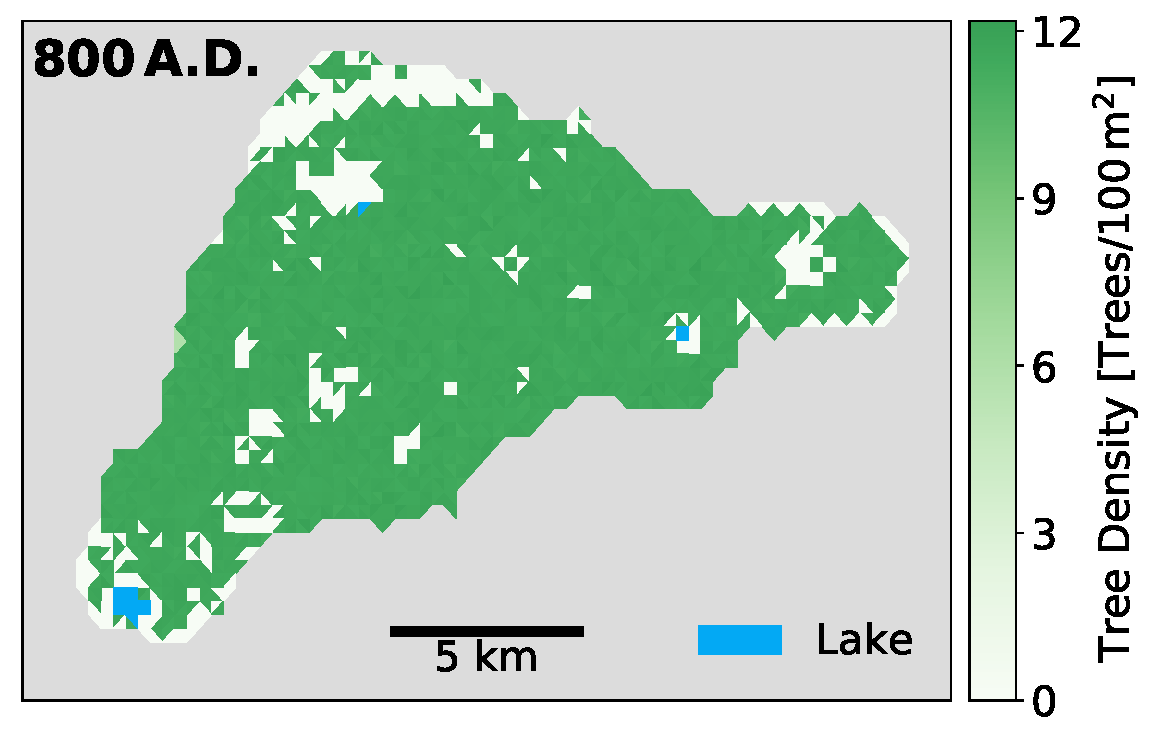
\includegraphics[width=\textwidth]{images/map_carrCap.pdf}
	\caption{The carrying capacity density of trees in each cell $T(c,t_\text{arrival})/A(c)$.}
	\label{fig:Map_tree}
\end{figure}

Through anthropogenic deforestation, the variable tree number in each cell, $T(c,t)$, declines.
The importance of this human influence in degrading the environment compared to the impact made by a quickly increasing number of Polynesian rats is a strongly debated topic (e.g.\ \citet{Bahn2017} and \citet{Hunt2007}) as described in the Introduction.
However, there seems to be a consensus between both theories that rats effectively hindered tree regeneration by gnawing on the palm nuts.
In line with these arguments, forest regeneration is not possible in the standard setting of this model.
Thus, trees constitute an entirely non-renewable resource in this scenario. 
However, I further explore alternative experiments in which the forest can hypothetically regenerate following anthropogenic deforestation.
Each year, tree numbers $T(c,t)$ in all cells $c$ regrow logistically to their (local) carrying capacity $T(c,t=t_\text{Arrival})$ if there is no farming activity on the specific cells.
The maximum growth rate of this localised logistic tree regeneration is believed to be rather slow and has even been made responsible for the ecological degradation of the island in earlier studies (e.g.\ \citet{Brander1998}).
\citet{Brandt2015} use a maximum tree regrowth rate between $0.02$ and $0.07 \, \rm{1/yr}$ for their model in the absence of rats.
In experiments, in which tree regeneration is allowed in this model, the maximum logistic growth rate is 
\begin{equation}
g_{\rm T} = 0.05\, \rm{1/yr} \ .
\end{equation}
Some cells are deforested entirely in a single update step, disabling their regeneration in the model. 
However, forest regrowth is also possible in such cells with seeds being transported to the empty cell e.g.\ through wind, birds or human activity.
To incorporate this in the model, a small number of trees `pops up' ($0.5\%$ of the cell's carrying capacity) after a cell has been left barren, i.e.\ the cell has been without trees and any farming activity, for $10$ consecutive years.
In summary, in this model the tree number in a cell $c$ either (standard setting) does not regenerate at all or (alternative setting) regenerates as
\begin{equation}\label{eq:treeupdate}
T(c,t+1)= \begin{cases}
T(c,t) + T(c,t) \cdot g_{\rm T} \cdot \left(1- \frac{T(c,t)}{T(c,0)}\right) \quad & \forall \ c \text{ with } \mathbf{A}_{\rm F}(c,t)=0 \\
0.005 \cdot T(c,0)  & \forall  \ c \text{ with } T(c,t)=0 \text{ and}\\
& \mathbf{A}_{\rm F}(c,\hat{t})=0 \  \ \forall \  \hat{t} \in \{t-10, \ldots, t\} \\
0 & \text{ else }
\end{cases}
\end{equation}
(neglecting anthropogenic deforestation).
These two scenarios, without and with forest regeneration, allow for testing of the impact of the Polynesian rats, assuming that they effectively hindered tree regeneration.

%Topic: Agriculture Yield
The Easter Island society also cultivated renewable crops as an alternative to harvesting the non- or slowly renewable trees.
Hence, agents in this model also farm on arable land in a two resource dependency similar to previous models \citep{dAlessandro2007}.
Farming produce in this model means in particular sweet potato cultivation, since this was the dominant staple crop \citep{Louwagie2006} (at least in the later part of pre-historic times).
As described in the Introduction, Easter Island's suitability for farming, especially w.r.t.\ climate and soil, has been subject to excessive debate.
While the total potential of agricultural productivity remains uncertain, several studies identified arable sites by using data on rain, climate, temperature, elevation and soil quality in agricultural models (e.g.\ \citet{Louwagie2006} and \citet{Puleston2017}).
The quality of farming and soil suitability on Easter Island and its spatial dependency is an ongoing research field, with crucial implications for the peak population size \citep{Puleston2017}.
The parametrisation of farming productivity shown in the remaining section, thus, is a strong limitation on the population dynamics.

In order to obtain a spatially explicit differentiation between arable and non-arable land, I use a map created by \citet{Puleston2017} (Figure 4) indicating regions meeting a certain viability criterion for sweet potato cultivation.
This criterion is based on an agricultural model of climate data and soil quality and marked $19\%$ of the island as agriculturally viable, mainly in the lowland, coastal region.
However, widespread systems of gardens were also found in the upland regions classified as non-viable by \citet{Puleston2017}'s criterion.
The authors state that these gardens added only a small fraction of actually farmed land to the viable region, though.
Here, I use three levels of viability for cells of the discretised map: 
A cell is either `well-suited' if located in the viable region, `poorly suited' if located in the non-viable region which was nevertheless farmed, or `non-viable' else (cp.\ with \citet{Puleston2017} (Figure 4)).
The total resulting arable land area in this model (shown in Figure \ref{fig:Map_agric}) is ca.\ $29\,  {\rm km^2}$ (i.e.\ $18\%$) for well-suited sites and, additionally, $50\, {\rm km^2}$ (i.e.\ $31\%$) for poorly suited sites.
%This fraction of arable land is in line with several different estimates from e.g.\ \TODO \citet{Bahn2017}???
%. TODO SOMEONE SAID THAT 50\% of the land was cultivated?

I distinguish well-suited from poorly suited cells by assigning different Farming Productivity Indices, $F_\text{PI}(c)$, for dryland farming to associated cells.
\citet{Louwagie2006} developed a classification for successful cultivation of several crops based on climate and soil property measurements at a few sites on the island and assigned classes of relative yields to them. 
One of the studied sites (Vaitea), which coincides with the poorly suited region in \citet{Puleston2017} (compare Figure 1 of \citet{Louwagie2006} with Figure 4 of \citet{Puleston2017}), was found not suitable for farming due to insufficient nutrition availability (with a relative yield of $0-20\%$ compared to an optimal site) despite archaeological evidence of gardens in this area.
To enhance yields, the islanders used techniques like labour intensive, large-scale lithic mulching, which mainly increased moisture availability, and efficient crop management, e.g.\ plant spacing and frequent fallowing \citep{Louwagie2006}.
The per area productivity, however, remains low even with these techniques in place with nutrient availability being the main constraint as also implied by the analysis in \citet{Puleston2017}.
The other sites in \citet{Louwagie2006} located at the foots of smaller craters along the arable coasts, were classified as mostly `marginally to moderately suitable' for sweet potato cultivation for most climatic conditions with some locations showing `high suitability' (relative yield $>80\%$) especially in wet years. 
These sites are mainly located in the well-suited or poorly suited regions of the map in \citet{Puleston2017}.
Hence, following roughly the classification by \citet{Louwagie2006}, a Farming Productivity Indices, $F_\text{PI}(c)$ is assigned to each cell (and its corresponding sites)
\begin{eqnarray*}
	F_\text{PI}|_\text{well} & = 80\% & \text{ for well-suited (highly to moderately suitable)}\\
	F_\text{PI}|_\text{poor} & = 10\%  & \text{ for poorly suited (not suitable)}\\
	F_\text{PI}|_\text{non-viable} & = 0\% & \text{ for non-viable sites}
\end{eqnarray*}
depending on its classification by \citet{Puleston2017} into well-suited and poorly suited cells.

Soil erosion through radical deforestation and heavy rainfalls also constrain the farming productivity of the island especially in the later phase (e.g.\ \citet{Brander1998}, \citet{Mieth2005}, \citet{Bahn2017}, \ldots).
As trees are removed from a region, rain can wash away nutrient-rich soil and reveal less fertile ground with reduced relative yield \citet{Mieth2005}.
In the model, I assume that, as a well-suited cell is completely deforested, the land erodes and, thus, the cell's $F_\text{PI}(c)$ reduces to 
\begin{equation}
F_\text{PI}|_\text{eroded}=50\% \quad \text{for well-suited cells with } T(c,t)=0 \ .
\end{equation}
This soil degradation is reverted as soon as trees pop back up (i.e.\ if the cell has been kept barren (without farming) for the previous $10$ years as described in equation \ref{eq:treeupdate}).

Throughout the simulation, agents set up basic unit gardens of size $1\, {\rm acre}$ on arable (well-suited or poorly suited) cells.% and obtain a farming produce according to the cell's farming productivity index.
A cell on arable (i.e.\ well-suited or poorly suited) land has
\begin{equation}
A_{\rm acres}(c) = \text{Rounded Down }(A(c)[\text{acres}])
\end{equation}
number of acres, which are denoted as sites and can each be occupied and farmed by an agent.
Such a farming site yields a produce according to the (relative) Farming Productivity Index, $F_\text{PI}(c)$.
The absolute productivity of an acre of arable land in units of people it can support is taken from calculations in \citet{Puleston2017} assuming two different Nitrogen fixation scenarios (see in detail later).
The map of Farming Productivity Indices $F_\text{PI}(c)$ of all cells on Easter Island is shown in Figure \ref{fig:Map_agric}, thus defining where agents have access to farming and how productive farming would have been in this location in the model. 

\begin{figure}
	\centering
	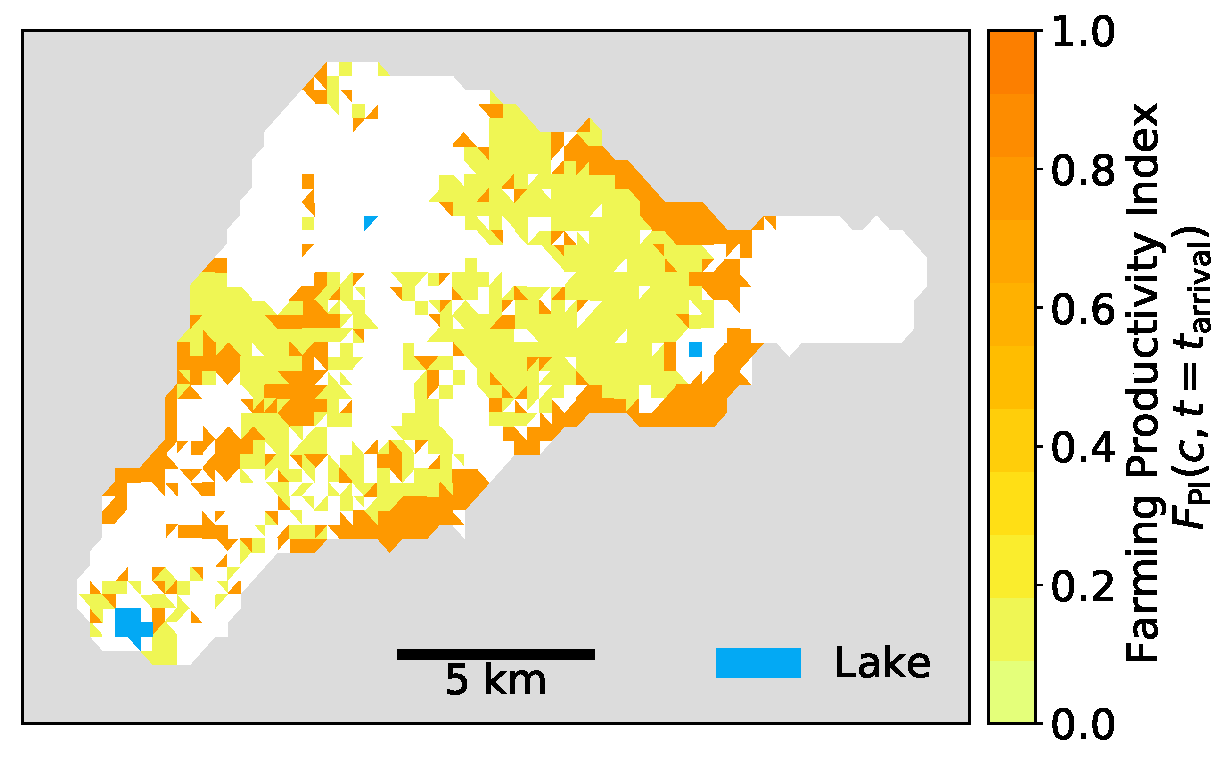
\includegraphics[width=\textwidth]{images/Plot_F_PI_c.pdf}
	\caption{A map of the (sweet potato) Farming Productivity Indices, $F_\text{PI}(c)$, in each cell of the discretised map of Easter Island. The model makes use of the map of \citet{Puleston2017} classifying arable land into viable areas (here `well-suited sites'), non-viable but nevertheless partially farmed (here `poorly suited sites'), and non-viable sites derived from an agricultural model of climate and soil quality. 
	This classification is combined with measurements of land suitability in several sites \citep{Louwagie2006} giving rise to a simple, spatially explicit map of farming potential parametrised by the Farming Productivity Index $F_\text{PI}(c)$.}
	%The Farming Productivity Indices in areas where gardening was observed but that did not meet the agricultural potential of \citet{Puleston2017}'s criterion is $10\%$ in line with the result of a model of agricultural yield from measurments in one such site by \citet{Louwagie2006}.}
	\label{fig:Map_agric}
\end{figure}


\section{Agents and Agent-Environment Interaction}\label{sec:AgentUpdate}
% Topic: Agents Households with properties
\subsection{Agent Properties}\label{sec:agentprops}
The ABM consists of a variable number of agents, $N_{\rm Agents}(t)$, which represent households, situated on the discretised map derived in Section \ref{sec:CreateMap}.
An agent with index $i$ has several varying properties describing its state at time $t$.
The settlement is located at 
\begin{equation}
	\vec{x_{\rm i}}(t) = (x_{\rm i},\, y_{\rm i})(t)
\end{equation}
 on the discretised map and, hence, associated with one specific cell $c_{\rm i}(t)$.
 The agent's population size, i.e.\ the number of individuals in the household, 
 \begin{equation}pop_{\rm i}(t) \end{equation}
 typically ranges from $12$ (minimum $6$) to ca.\ $42$.% ranging from $6$ to $42$ .
While, all calculations and decisions on harvest and choosing a settlement location happen on the individual level, macroscopic aggregates are simply obtained by iterating over all agents, which I denote by bold symbols in the thesis (same as for iterating over cells). 
%Iterations over all agents (or cells of the map for the corresponding variables) are denoted via bold symbols in all equations in this thesis.

Agents rely on an intake of resources each year in order to sustain and potentially increase their population size.
As mentioned before, I consider two major resources, trees and sweet potato farming, accessible through interaction with the environment.
An agent $i$ can harvest resources from cells with midpoints $\vec{\tilde{c}}$ located within fixed radii of the agent's settlement:
\begin{equation} \label{eq:Circle_T}
C_{T}(c_{\rm i}(t)) = \{ \tilde{c}\ | \   | |  \vec{\tilde{c}} - \vec{x_{\rm i}}(t) | |  \leq r_{\rm T} \} 
\end{equation}
for the resource tree with tree search radius $r_{\rm T} =2\, {\rm km}$ and 
\begin{equation} \label{eq:Circle_F}
C_{F}(c_{\rm i}(t)) = \{ \tilde{c}\ | \   | |  \vec{\tilde{c}} - \vec{x_{\rm i}}(t) | |  \leq r_{F} \}
\end{equation}
for farming sites with farming radius $r_{\rm F} = 1\, {\rm km}$.

The agent's total resource uptake is split between tree cutting and farming yield.
The shares are given by a trait parameter, the tree preference $T_\text{Pref, i}(t)$ for agent $i$ at time $t$, which adapts the agent's harvest behaviour to its local environment.
In the first settlement phase, the islanders mainly lived off the abundant natural resources of the island, i.e.\ land birds, fish, and fruits from the trees \citet{Bahn2017} (which are all connected to the resource tree in this model). 
Over time, the economy `switched from predominantly hunter-gatherer to a dryland farming society' \citep{Louwagie2006}.
In the model, this behavioural shift results from a decrease in the variable tree preference parameter, $T_\text{Pref, i}(t)$ of each agent over time.
The trait parameter is designed such that agent's adjust their resource requirements for next year given the current state of the local environment, in particular the level of deforestation. 
%It is an adaptive trait reflecting the local state of the environment around an agent, in particular the local abundance of trees. %(i.e.\ trees $T(c,t)$ of cells within $C_{\rm T}(c_\text{i}(t)$).
Hence, as the island's trees are removed and more arable land is cleared freeing space for agriculture, the agent's tree preference decreases and farming activity increases, accordingly.
%This tree preference indicates the value of tree harvest over agricultural production and, hence, increases the need for one over the other in order to fill the resource requirements.
%The tree preference is high in the initial state, but decreases as trees become scarce and more land is available for cultivation of crops.
%Hence, $TPref_{\rm i}(t)$ responds to some degree to the local environment of the agent.
In this model, the tree preference, $T_\text{Pref, i}(t)$, depends on the local, relative change of tree density within the tree search radius $r_{\rm T}$ with respect to the initial state at $t=t_\text{arrival}$, i.e.:
\begin{equation}\label{eq:TPref}
T_\text{Pref, i}(t) = f_\text{Tree Pref}\left( \, \frac{\sum_{\tilde{c} \in C_{T}(c_{\rm i}(t)) } \, T(\tilde{c}, t)}{\sum_{\tilde{c} \in C_{T}(c_{\rm i}(t))} \, T(\tilde{c}, t_\text{arrival}) } \, \right)
\end{equation}
The shape of the function $f_\text{Tree Pref}$ is an indicator of the responsiveness of the economy/society to environmental change. How fast do agents adapt their harvest behaviour, when the non-renewable resource, the trees, is depleted from the initial state?  
I consider four possibilities (shown in Figure \ref{fig:TPref_T}): The tree preference $T_\text{Pref, i}(t)$ decreases
\begin{itemize}
	\item linearly with the local, relative tree density decline (linear case).  
	\item delayed with the local, relative tree density decline (delayed case).
	\item quicker than the local, relative tree density decline (careful case),
	\item first delayed, and at some point quicker than the local, relative tree density decline (logistic case) 
\end{itemize}
\begin{figure}
	\centering
	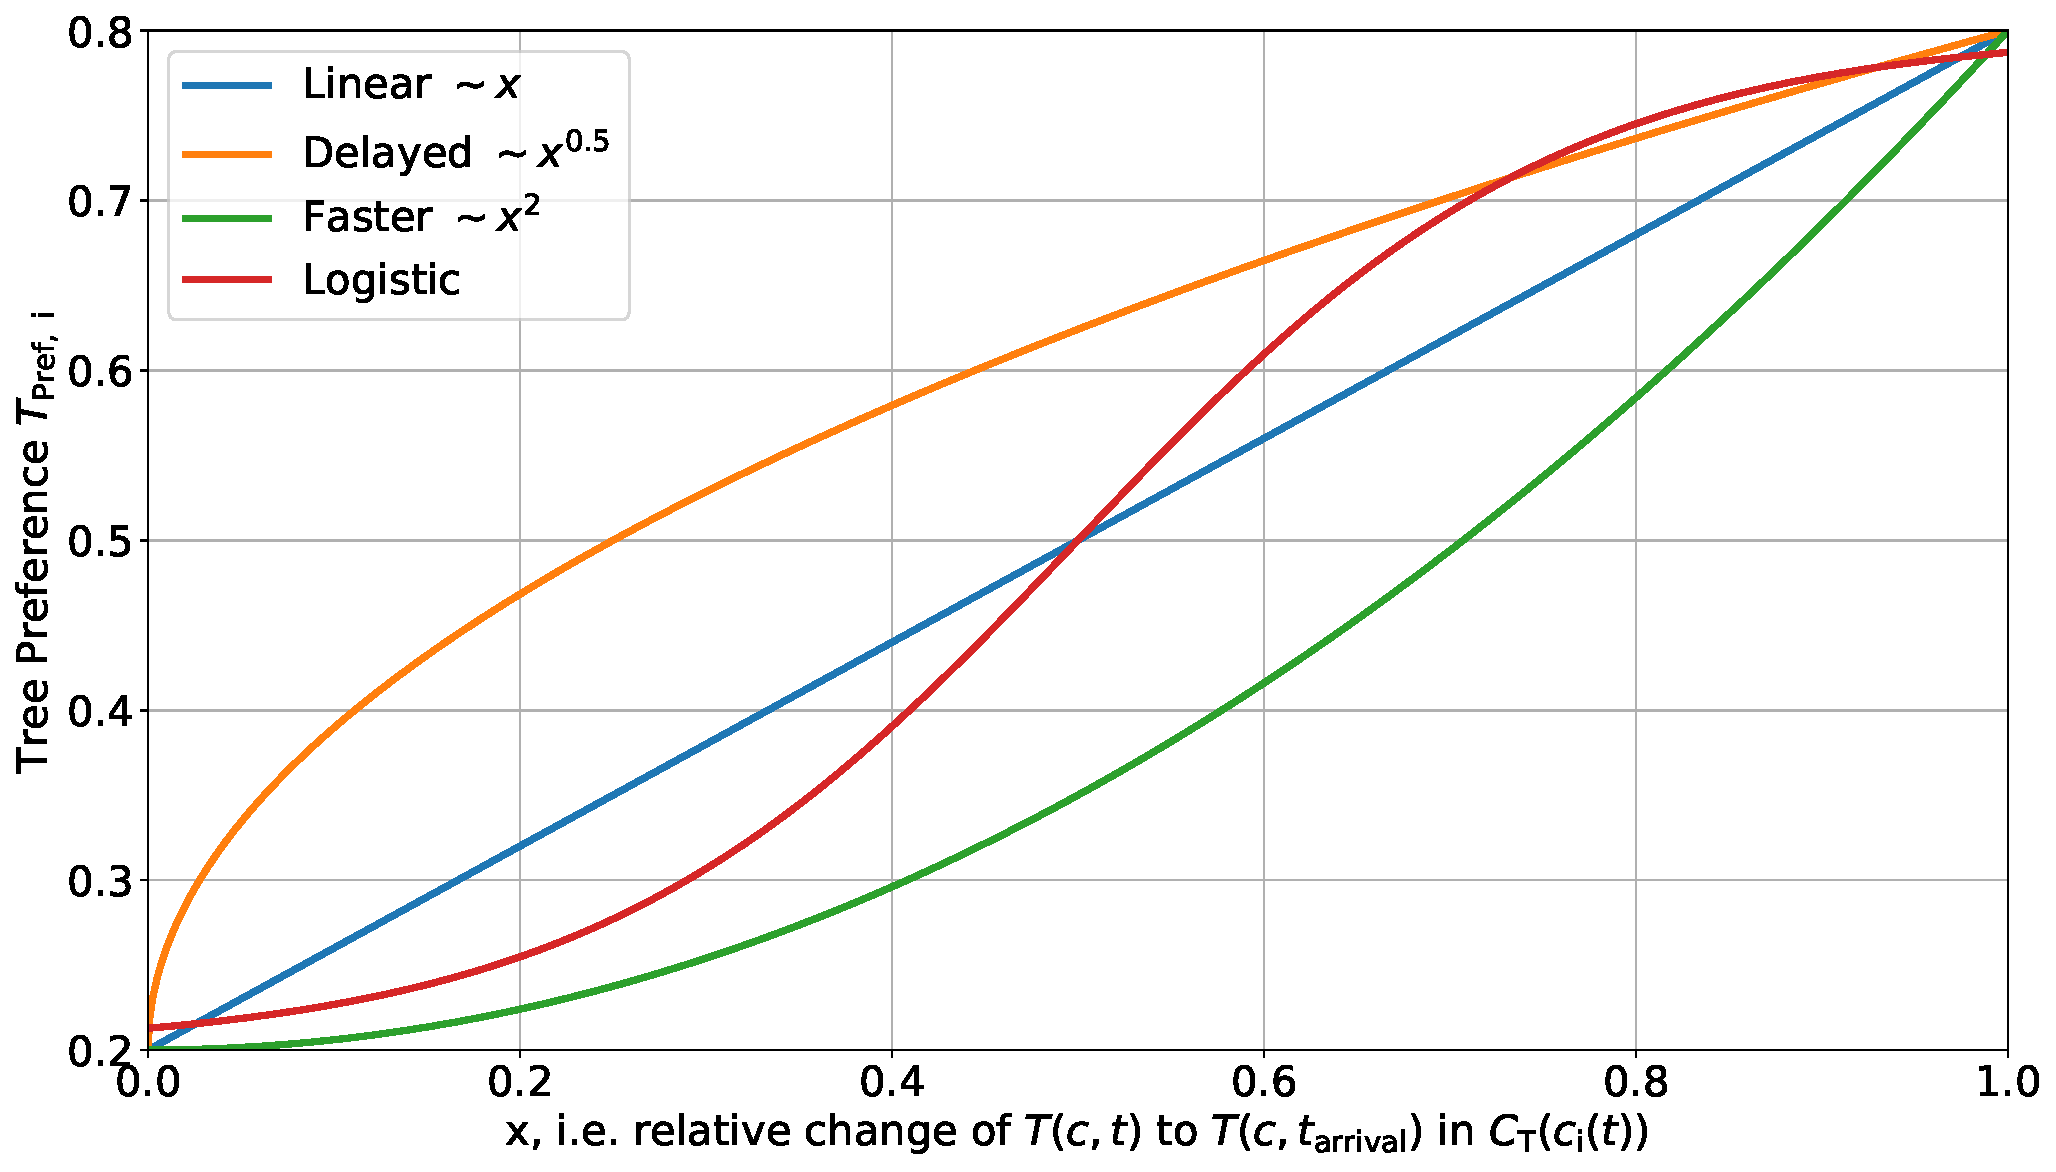
\includegraphics[width=\textwidth]{images/TPref}
	\caption{The relation of an agent's tree preference, $T_\text{Pref, i}(t)$, to relative changes in the local tree density for the four considered adaptive functions $f_\text{Tree Pref}$ with $x$ given in equation~\ref{eq:TPref}.}
	\label{fig:TPref_T}
\end{figure}
The tree preference is cut off at certain minimum and maximum thresholds, assuming an agent can not live purely off trees (and associated derivative products), but, at the same time, some tree cutting is always required even for maximum agricultural production (e.g.\ as cooking wood or for tools). 
Here, I choose: 
\begin{equation}
T_\text{Pref, min} = 0.2 \quad \text{and} \quad T_\text{Pref, max} = 0.8
\end{equation} 
In the standard setting in this model, I use the linear relation and, hence, 
\begin{equation}
	T_\text{Pref, i}(t) =  \frac{\sum_{\tilde{c} \in C_{T}(c_{\rm i}(t)) } \, T(\tilde{c}, t)}{\sum_{\tilde{c} \in C_{T}(c_{\rm i}(t))} \, T(\tilde{c}, t_\text{arrival}) } \cdot (T_\text{Pref, max}-T_\text{Pref, min}) + T_\text{Pref, min}
\end{equation}
Since tree density is maximal at $t=t_\text{arrival}$, the initial agents start with maximal tree preference ($T_\text{Pref, i}(t=t_\text{arrival}) = 0.8 \ \  \forall \ i$), which then (in general) decreases as the (local) deforestation intensifies.

An agent's required total resource uptake per year increases with the population size and the tree preference calculated after the harvest in the previous year.
Hence, the resource requirements of tree harvest, $T_\text{Req, i}(t)$, and farming produce, $F_\text{Req, i}(t)$, are 
\begin{equation}
T_\text{Req, i}(t) = T_\text{Pref, i}(t-1) \cdot pop_{\rm i}(t) \cdot T_\text{Req, pP} \, 
\end{equation}
and, similarly, 
\begin{equation}
F_\text{Req, i}(t) = (1-T_\text{Pref, i}(t-1)) \cdot pop_{\rm i}(t) \cdot F_\text{Req, pP}\, , 
\end{equation}
where $T_\text{Req, pP}$ is the tree requirement per year per person in absence of agriculture and $F_\text{Req, pP}$ is the required agriculture production per year in the absence of tree cutting.
These constant parameters determine the amount of tree harvesting and farmland occupation and, thus, are crucial for the temporal development of the island's environment. 

The tree requirement per person, $T_\text{Req, pP}$, in principle depends on a multitude of factors and is presumably heterogeneous between agents.
E.g.\ if sugary sap from cut tree trunks was used by some people as freshwater replacement as suggested by \citet{Mieth2015}, a much larger number of trees would have been needed to cut by those individuals.
Here, I use a constant parameter of 
\begin{equation}
T_\text{Req, pP} = 5\, \frac{\text{Trees}}{\rm person\cdot yr}
\end{equation}
for all agents (for the standard model settings) based on the maximum harvest rate used in \citet{Brandt2015}, ca.\ $3$ to $7$ trees per year\footnote{\citet{Brandt2015} use a only half of the initial trees before arrival of the first settlers, though)}. 
%In the standard run I am using $5$ Trees per Person per year. However, I vary this parameter in a sensitivity analysis (see Section \ref{sec:SensitivityAnalysis}).

The agriculture requirement per person, $F_\text{Req, pP}$, is strongly connected to the definition of the farming productivity indices $F_\text{PI}(c)$ (Figure \ref{fig:Map_agric}).
\citet{Puleston2017} simulate the nutritional productivity of farming on well-suited land (as defined in Section \ref{sec:CreateMap}) for two different environmental scenarios for the Nitrogen fixation in the soil, i.e.\ the rate at which Nitrogen is renewed, representing a major uncertainty in their model.
This can be converted into the minimum land required to sustain one person using the nutrition content of sweet potato ($1\, \rm{t/yr}$ roughly sustains $1$ individual in the absence of other food sources): 
\begin{equation}
F_\text{Req, i}(t) = \begin{cases}
	0.5 \, {\rm \frac{acre}{person} } & \text{ for high N fixation} \\
	1.7 \, {\rm \frac{acre}{person} } & \text{ for low N fixation} \\
 \end{cases}
\end{equation}
%For $AReq\_pP$, I am using the estimates by \citet{Puleston2017}. In their agricultural model, they identify the Nitrogen fixation as a major uncertainty in the evaluation of potential agricultural yields. 
%With two different assumptions of Nitrogen fixation in the soil (high and low), \citet{Puleston2017} model the sweet potato harvest on a high quality agriculture site and combine it with the nutritional need of an individual person.
In this model, I do not consider fallowing as farming practice to increase productivity of arable land, as this, in general, reduces the productivity per total occupied area needed for each individual (see Table 1 in \citet{Puleston2017}).
In fact, the only constrain for farming is availability of arable land in this model, not workforce or any social/political constraints (as included in \citet{Puleston2017}).
I.e.\ I assume that, if enough land is available, the agent's occupy as many sites as necessary.
%One can then calculate that for high N-fixation for one person (in the abesence of other food) needs $0.5\, \rm{acres}$ of high quality agricultural productivity of sweet potato cultivation.
%In the case of low N-fixation this increase to $1.7\, \rm{acres}$ per Person. 
%Here, I am using both values in order to test the different scenarios.
Hence, the resource requirements for trees (in absolute numbers) and agricultural production (in acres of well-suited quality agriculture sites) are agent-specific, yearly varying features, which can be tuned through the global parameters $T_\text{Req, pP}$ and $F_\text{Req, pP}$.

% Topic: Fishing Agents constrained by a tabu 
The model, furthermore, allows for open-ocean fishing as a replacement for farming for some agents living near the Anakena coast.
Instead of occupying arable land units and farming, these fishers gain sufficient agricultural resources by going out to sea on large canoes.
In the initial phase of Easter Island settlement, excavations prove that shellfish, fish and even porpoise were a major part of the diet at the time \citep{Bahn2017}.
However, over time, these natural resources became increasingly scarce and many species even went extinct due to human predation, with open-ocean fish vanishing from the diet eventually \citep{Diamond2011}.
As a resource management institution the Easter Island society installed taboos on the harvest of natural resources \citep{Good2006}. 
Fishing was mainly restricted to members of a specific chiefdom (`Miru') living at Anakena Beach \citep{Bahn2017} who would then presumably trade with others.
%According to \citet{Bahn2017} or \citet{Diamond2011}, sea fish vanished from the Easter Island typical diet by \TODO.
Hence, in the model, every agent living within farming radius, $r_{\rm F}$, distance of Anakena Beach (in cell $c_{\rm Anakena}$) automatically becomes a fishing agent up to a maximum of $N_\text{Fisher, Max} = 10$ agents in total (i.e.\ no more than $500$ people)
\begin{equation}
 	c_{\rm i} \in C_{\rm F}(c_{\rm Anakena}) \  \cup \ N_\text{Fishers}<N_\text{Fisher, Max} \quad \Rightarrow \text{Agent }i\text{ becomes a fisher}
\end{equation}
%At time $t_\text{taboo fishing}=$\TODO a taboo is put in place externally.
%Consequently no new fishing agent's are accepted .
% letting only \TODO those agents already pursuing fishing to continue but allowing no further agents to enter this resource stock. 
While I assume that open-ocean fish supply is unlimited for those living at Anakena Beach, another constraint for the fishers is the requirement for trees.
Since fishing presumably requires a quite extensive amount of wood (e.g.\ for canoes or firewood), the fishers minimum tree preference is increased to
\begin{equation}
T_\text{Pref, min}|_\text{fisher} = 0.5
\end{equation} 
rather than $T_\text{Pref, min} = 0.2$ for farming agents.
While fishing agents near Anakena Beach do not have any farming requirements due to their access to an unlimited resource stock from the sea, the correspondingly higher requirement for trees and an externally introduced restriction on their number limit the total amount of this resource extraction.

\subsection{Agent-Environment Interaction -- Tree and Agriculture Harvest} \label{sec:Harvest}
% TOpIC: HARVEST GENERAL
After determining the required amount of trees, $T_\text{Req, i}(t)$, and agricultural production, $F_\text{Req, i}(t)$, as described in Section \ref{sec:agentprops}, in a given year $t$, an agent acquires sufficient resources (if available) from its local environment.
This procedure is described in the remaining section. 
The sketch in Figure~\ref{fig:treeburning} shows an example of this process of deforestation and consequent replacement by farming in a cell.
\begin{figure}
	\centering
	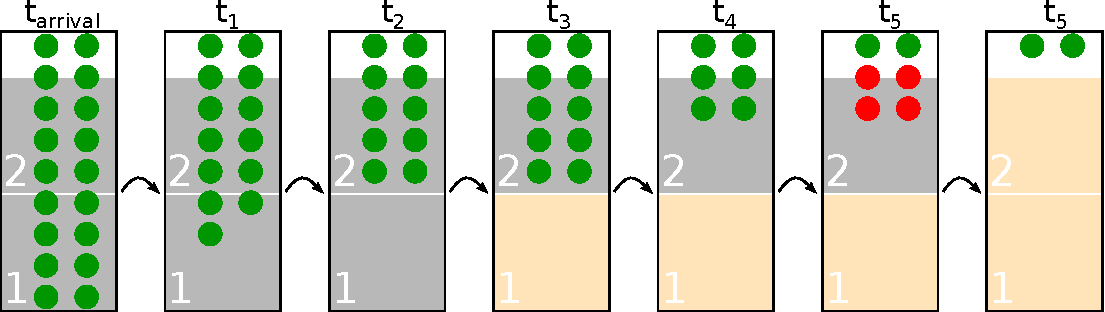
\includegraphics[width=\textwidth]{images/SketchABM2/burningSketch.pdf}
	\caption{Sketch of an exemplary deforestation procedure (by arbitrary agents) in a cell $c$ (black box) with an area of $2.3\, \rm{acres}$.
		The cell is arable, with $F_{\rm PI}(c)>0$ and, thus, provides $A_{\rm acres}=2$ acres for potential farming (grey squares).
		Initially at $t_{\rm arrival}$, the cell has $18$ trees (carrying capacity).
		At some time $t_{\rm 1}$, after deforestation $13$ of these trees still exist. 
		An Agent $a$ removes $3$ trees from the cell (\ra $t_{\rm 2}$). 
		Subsequently, Agent $b$ then occupies the now cleared site ($1\, {\rm acre}$) on cell $c$ for farming (\ra $t_{\rm 3}$). 
		Agent $c$ cuts another $4$ trees (\ra $t_{\rm 4}$).
		And finally, at $t_{\rm 5}$, an agent $d$, needs to occupy more sites to fill its farming requirement and cannot find any other arable, unoccupied site in $C_{\rm F}(c_c)$ except for the second site in cell $c$. 
		However the agent needs to burn $4$ more trees (red) before being able to occupy the second acre on this cell (\ra $t_{\rm 5}$).}
	\label{fig:treeburning}
\end{figure}

\paragraph{Farming}
An agent occupies arable land unit sites, $A_\text{F, i}(t)$, with a fixed area of $1\, \text{acre}$ associated to one cell and obtains a yearly harvest of
\begin{equation}\label{AProd}
F_\text{i}(t) = \sum_{a \, \in \, A_\text{F, i}(t)} \, F_{PI}(c(a))\ ,
\end{equation}
where $a$ denotes a farmed acre and $c(a)$ is the corresponding cell of this acre.
Note, for fishers $F_\text{i}(t) = F_\text{Req, i}(t)$ holds immediately without farming and occupying sites.
Agents keep all their currently occupied sites $A_\text{F, i}(t)$ until the next year.%, i.e.\ $acres_{\rm i}(t+1) = acres_{\rm i}(t) + new\_acres(t+1)$.
However, over time, the agents farming requirement, $F_\text{Req, i}(t)$, can increase as the agent's population grows, its tree preference decreases or the soil quality of an agent's occupied sites degrades due to erosion.
Hence, an agent $i$ needs to acquire more arable sites only if the requirement for farming, $F_\text{Req, i}(t)$, exceeds the farming produce of the previous year, $F_\text{i}(t-1)$, i.e.\
\begin{equation}
F_\text{i}(t-1) < F_\text{Req, i}(t) \ \Rightarrow \ \text{Extend } A_\text{F, i}(t) \text{ and, thus, } F_\text{i}(t) {\rm !}
\end{equation}
%Then the agent occupies more sites extending $A_\text{F, i}(t)$ and, thus, increasing the produce $F_\text{i}(t)$ accordingly.

In the search for new farming sites, an agent first considers only sites in well-suited cells, i.e.\ $c \in C_\text{F}(c_\text{i}(t))$ with $F_\text{PI}(c)=F_\text{PI}|_\text{well}$, in order to maximise farming efficiency.
An acre in an arable cell can only be occupied (or added to $A_\text{F, i}(t)$) if at least this area of $1\, {\rm acre}$ is cleared off trees and not occupied. 
Assuming that the trees are evenly distributed on the cell's area, the condition can be calculated as 
\begin{eqnarray}
%& \text{Treeless Area\,[acre]} - \text{Occupied Acres\,[acre]}  & \geq 1  \\
%\Leftrightarrow & 
\left( 1 - \frac{T(c,t)}{T(c,0)} \right) \cdot A(c) - \mathbf{A}_\text{F}(c, t) & \geq   1
\label{eq:BurningCond}
\end{eqnarray}
where the first term is the treeless area in ${\rm acres}$ and the second term, $\mathbf{A}_\text{F}(c, t) = \sum_{j \in N_{\rm Agents}(t)} \, \sum_{a \, \in \, A_\text{F, j}(t)} \, \delta(a=c)$, is the number of already farmed acres (by any agent) in cell $c$.

If there are no well-suited sites left that fulfil this condition, the agent uses the slash and burn method to reduce the number of trees $T(c,t)$ of a well-suited cell $c$ (with at least one unoccupied acre).
The agent starts burning trees on the cell that requires the least amount of trees removed (without leading to erosion of the cell) for the condition to hold.
Burning trees and occupying sites continues until the farming requirement of the agent is satisfied or no more well-suited acres are available (even if this leads to erosion of the cell).
The use of fires to clear space is supported by the extensive charcoal record starting with the period of intensified agriculture \citep{Mieth2015}. 
Here, I assume that if space is required for farming, trees were burned directly and independently of the continuous tree harvest .
Of course, an agent could also use these trees first and (e.g.\ for extracting the sugary sap) then burn the remaining material to clear the land for next year as indicated by \citet{Mieth2015}, but this would require agents that plan ahead, which I do not consider in the harvesting process.
%felled and used (e.g.\ for extraction of the sugar sap) before burning and consequent agricultural use of the land \citep{Mieth2015} or slash and burn method was used directly to clear space as necessary next to tree harvest %(e.g.\ indicated by \citet{Bahn2017}). % Bahn: ``fires directly accompanied by agriculture''
If, all well-suited sites within $C_{\rm F}(c_{\rm i}(t))$ are occupied, but the agent's agricultural production does not yet meet the farming requirement ($F_\text{i}(t)<A_\text{Req, i}(t)$), the agent also occupies sites on eroded cells and then on poorly suited cells in the same procedure.


\paragraph{Tree Harvest}
After filling the farming requirement, the agent then cuts trees according to its tree requirement $T_\text{Req, i}(t)$.
An agent $i$ selects random cells $c\in C_{\rm T}(c_{\rm i}(t))$ with uniform probabilities and successively removes trees from these cells until the number of cut trees, $T_\text{i}(t)$ matches the requirement $T_\text{Req, i}(t)$ or no further trees are present in $ C_{\rm T}(c_{\rm i}(t))$. 
Unlike farming, where occupied sites are kept and re-used (with the same productivity index) in the next update, the agent obviously needs to find new trees every year.
%Therefore, if tree regrowth is disabled, this tree harvest represents a non-renewable resource dependency of the Easter Island society.
While the agent's adapt their harvest behaviour via the tree preference as this non-renewable resource is depleted over time, a minimum amount of trees is always required and, hence, there's no equilibrium state without tree regrowth.

\paragraph{Happiness}
Agents have a variable happiness, $h_{\rm i}(t)$, that reflects the success of the harvest of trees and farming produce each year.
Here, an agent $i$'s happiness $h_\text{i}(t)$ depends on the ratio between the $T_\text{i}(t)$ cut trees and $F_\text{i}(t)$ agricultural produce in comparison to the requirements determined beforehand, $T_\text{Req, i}(t)$ and $F_\text{Req, i}(t)$, respectively.
%Assuming that both requirements determine  the tree requirement and the agriculture requirement is equally important to the agent, the happiness is simply the minimum of the fraction of requirements that could be filled:
By assuming that both resources are equally indispensable for the agent, the happiness is equal to the smaller of the two fractions:
\begin{equation} 
h_\text{i}(t) = {\rm min} \left( \frac{T_\text{i}(t)}{T_\text{Req, i}(t)}, \, \frac{F_\text{i}(t)}{F_\text{Req, i}(t)} \right)
\label{eq:h_i}
\end{equation}
If both requirements are filled for agent $i$, the happiness is maximal: $h_\text{i}(t)=1$.
However, if either $T_\text{i}(t)=0$ or $F_\text{i}(t)=0$, $h_\text{i}(t)=0$ follows regardless of the success in harvesting the other resource.
Since households have some resilience to a decline in harvest success (e.g.\ by storing food over more successful years), a memory happiness $H_\text{i}(t)$ is calculated in each year:
\begin{equation}
H_\text{i}(t) = \begin{cases} 
				h_\text{i}(t) & \text{ if } h_\text{i}(t)\geq h_\text{i}(t-1) \\
				\frac{h_\text{i}(t) + h_\text{i}(t-1)}{2} & \text{ if } h_\text{i}(t)<h_\text{i}(t-1) 
		\end{cases}
\end{equation}
If an agent's harvest success decreases (due to resource scarcity), its memory happiness $H_{\rm i}(t)$ decreases monotonically.
If e.g.\ all trees were to suddenly vanish within a year, an agent would have two years before its memory happiness plummets to its minimum $H_\text{i}(t) = 0$.
However, if harvest success increases (e.g.\ due to moving the settlement to a better location), the memory happiness takes on the new happiness value immediately.
As an indicator for successful resource acquisition, the memory happiness $H_\text{i}(t)$ determines the possible responses of agent $i$ to the harvest, which I describe in the following Section \ref{sec:Reaction}.

\section{Agent's reaction to the harvest}\label{sec:Reaction} 
\subsection{Population Dynamics}
Following an agent's farming and tree cutting actions, its population size $pop_{\rm i}(t)$ is adapted. 
The net (positive or negative) growth rate of the agent's population at a specific time depends only on the memory happiness:
\begin{equation}\label{eq:popgrowthcontinuos}
pop_{\rm i}(t+1) = g(H_{\rm i}(t)) \cdot pop_{\rm i}(t)
\end{equation}
In fact, instead of assuming continuous growth or decline according to this growth rate, $g(H_{\rm i}(t))$, the population dynamics is implemented as a discrete, stochastic process.
Each individual member of the agent has a ${\rm abs}(g(H_{\rm i}(t))-1)$ probability to die if $g(H_{\rm i}(t))<1$, or a $g(H_{\rm i}(t))-1$ chance to reproduce (i.e.\ adding one individual to the household/agent) if $g(H_{\rm i}(t))>1$.
The population size stays constant if $g(H_{\rm i}(t))=1$, denoted as $H_{\rm equ}$. 
This results in a growth/decline of the population where each agent's population size trajectory is a single realisation of the stochastic process which on average matches the continuous dynamics in equation~\ref{eq:popgrowthcontinuos} (compare e.g.\ with \cite{Bungartz2009}).
Figure \ref{fig:realisationsofpopgrowth} in Appendix \ref{sec:APPpopgrowth} shows a few different realisations of a discrete, constant growth scenario with rate $g(H_{\rm i}(t)=1)=1.007$ (i.e.\ with unconstrained resource availability) in comparison with the continuous growth.

There is an excessive debate about the initial growth rate of the Easter Island population after the arrival of a small number of Polynesians (i.e.\ in a time period without resource constraints and, thus, $H_{\rm i}(t)=1$).
Parameters used in the literature range from $0.7\%$ per year \citep{Bahn2017} or `always below $1\%$' \citep{Brander1998} to exceeding $3\%$ \citep{Hunt2007} for short periods of time or $2.3-4.5\%$ \citep{Brandt2015}.
It is clear that depending on the proposed chronology, researchers have to make very contrary assumptions on the population growth in order to fit the population dynamics to the few undisputed facts about the pre-historic society on Easter Island. 
If an arrival around $1200\, \text{A.D.}$ is assumed (as in \citet{Hunt2007} or \citet{Brandt2015}), assuming a large population growth is unavoidable. 
It seems impossible that only a few hundred inhabitants in the 13th to 16th century could have created several hundred Moai statues (and caused a massive alteration of the island's environment).
On the other hand, slower initial population growth needs to be assumed in studies proposing earlier arrival dates (around $800\, \text{A.D.}$(e.g.\ \citet{Bahn2017}) or even as early as $400\, \text{A.D.}$ (\citet{Good2006} and \citet{Brander1998})), since archaeological data indicates an intensification of human activity, which suggests a large population size, only starting after $1200\, \text{A.D.}$ (e.g.\ \citet{Bahn2017}) and \citet{Hunt2007}).
Other theories, such as multiple, distinct periods of population growth and declines have been put forward (e.g.\ \citet{Cole2008}), but do not seem to be common in the context of Easter Island.
%Archaeological data, e.g.\ charcoal evidence, however, suggests a period of intensification of human activity starting after $1200\, \text{A.D.}$ (e.g.\ \citet{Bahn2017}) and \citet{Hunt2007}).
%Hence, these studies assume a slow but continued population growth starting with the `early' arrival.% way before $1000\, {\rm A.D.}$.% up to a peak population in $1300-1700\, \text{A.D.}$.
%, one has more freedom in choosing the initial growth rate.
%especially considering that there might have been several phases of population declines as proposed in \citet{\TODO Bahn2017}. 
%One could imagine that after initial fast growth of the population after an early arrival, through fertility control a steady population size was reached below Easter Island's resource carrying capacity. 
%Archaeological and charcoal data, however, suggest an intensification of human activity (and its impacts on the environment) only at around 1200 \citet{Hunt2007} and very little environmental impact before that.
%Most researchers rather assume a slow but continued population growth from an early arrival to a peak population around 1300-1700 (e.g.\ \citet{Brander1998}, \citet{Bahn2017})
Following \citet{Bahn2017}, I choose an early arrival date here ($t_\text{arrival}=800\, A.D.$), as described before, and, thus, a slow growth rate (in one year) in the case of unlimited food supply and, therefore, continuously happy agents: 
\begin{equation}
	g(H_\text{i}(t)=1) = 1.007 \ .
\end{equation}

The specific dependency of the population growth or decline in the case of limited resources is a further uncertainty in modelling human-resource interactions in general.
\citet{Lee2008} and \citet{Puleston2008} constructed a food-limited demography model applied to simulating the Easter Island society and farming constraints in \citet{Puleston2017}. 
Here I use a strongly simplified assumption of this model to parametrise the impact of non-optimal harvests on the population dynamics. 
The authors derived age-dependent survival and fertility rates, which are both S-shaped curves w.r.t.\ the food availability (i.e.\ high in the case of unlimited food availability and low in the case of scarce food availability).
Since, I do not consider (age-stratified) structures below the agent/household level, I simply assume a net growth rate with the same shape as the survival and fertility rates in \citet{Lee2008}.
\begin{equation}
g(H_\text{i}(t)) \sim CDF(\Gamma_\text{Dist}(shape, scale=0.1))
\end{equation}
where $CDF(\Gamma_\text{Dist})$ is the cumulative density function of the Gamma distribution (characterised by shape and scale parameter) with scale fixed as in \citet{Lee2008}.
I then tune the shape parameter of this function to obtain the same equilibrium point $g(H_\text{i}(t) =H_\text{equ})=1$, at which the population size remains constant, as in \citet{Puleston2017} (Supplementary Material):
\begin{equation}
H_\text{equ}=0.6883 \quad \text{with } g(H_\text{i}(t) = H_\text{equ})=1   \ .
\end{equation} 
In order to test sensitivity of this parametrisation, I also investigate a larger shape parameter $shape^*=3$, which leads to a less resilient population size when resource scarcity sets in.
In this alternative, less resilient scenario, the growth rate declines faster if $H_\text{i}(t)$ decreases and the equilibrium point is reached for a higher happiness value $H_\text{equ}^*=0.84$.  %$g(H_\text{i}(t)=H_\text{equ}^*)=1$
The amplitude of the resulting function (for both scenarios) is scaled to give the chosen reproduction rate under unconstrained food supply from last paragraph 
$g(H_\text{i}(t)=1)=1.007$.
Figure \ref{fig:growthrate} shows the resulting two parametrisations of population dynamics (standard setting in blue and less resilient setting in red) with the happiness regime for net growth, $H_\text{i}(t) > H_{\text equ}$ (with a maximum of $g(H_\text{i}(t)=1)=1.007$) and the regime for net decline of the population size, $H_\text{i}(t) > H_{\text equ}$.
%(for $H_\text{i}(t)>H_\text{equ}$, with a maximum of $g(H_\text{i}(t)=1)=1.007$) and decline (for $H_\text{i}(t)<H_\text{equ}$) .
\begin{figure}
	\centering
	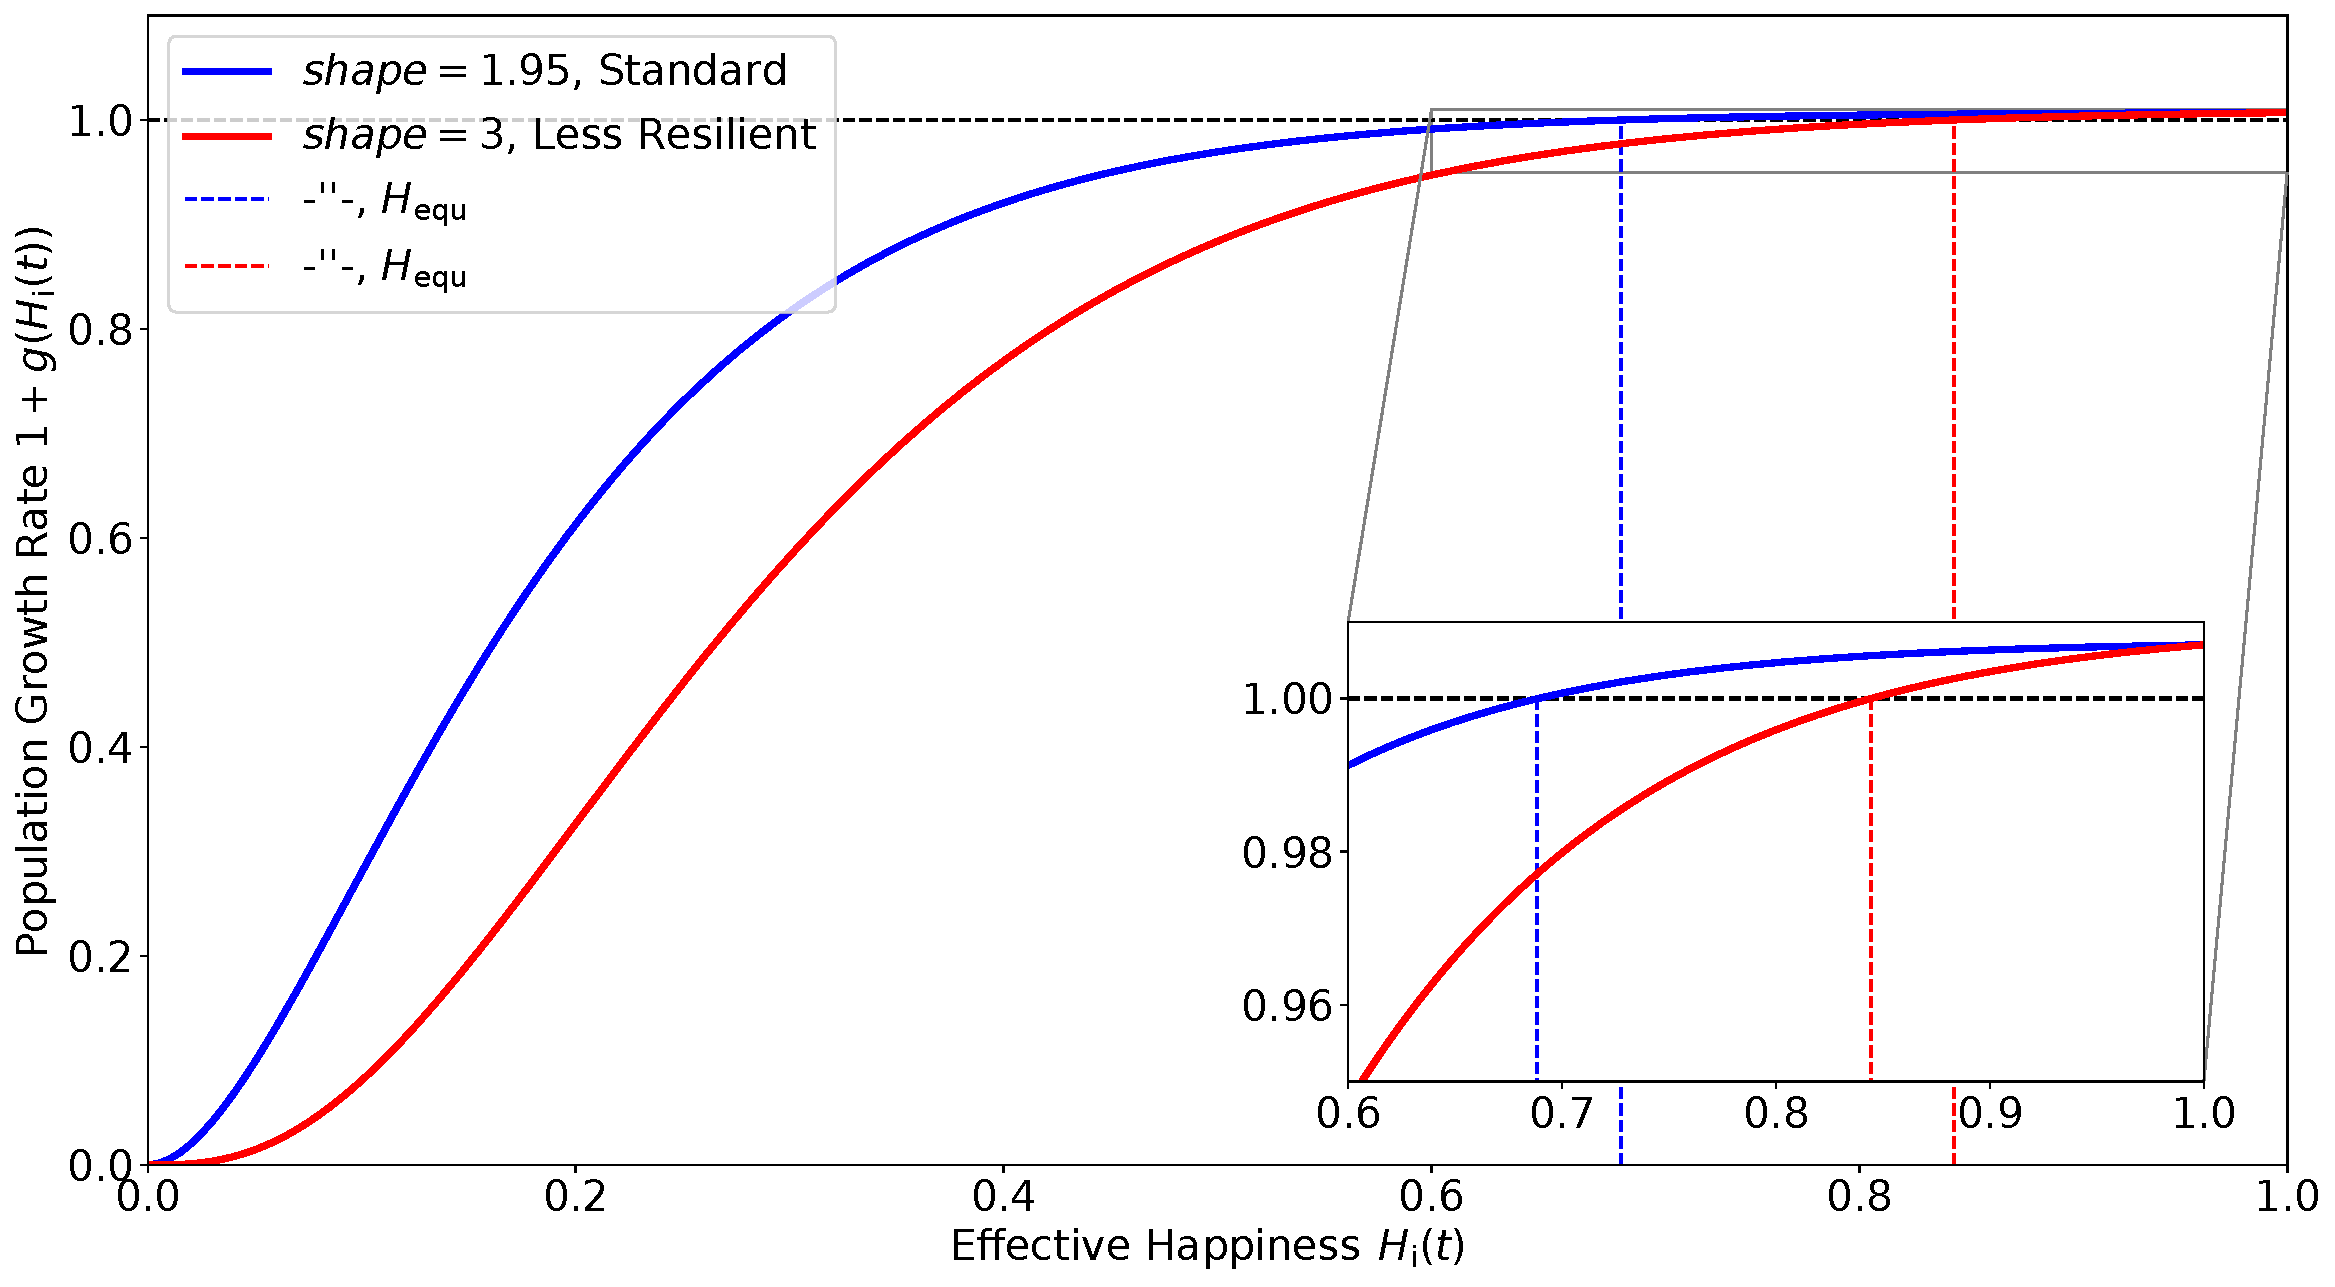
\includegraphics[width=\textwidth]{images/populationchange_g}
	\caption{The growth rate of an agent's population size as a function of its memory happiness $H_{\rm i}(t)$. Functional dependence follows simplified assumptions made in the food-limited demography model in \citet{Lee2008}, \citet{Puleston2008}, and \citet{Puleston2017}. In the standard scenario (red) the agent's population size grows if $H_{\rm i}(t)>H_{\rm equ}=0.6883$ and declines for smaller $H_{\rm i}(t)$. An alternative, less resilient scenario is also tested, with a smaller population growth regime of $H_{\rm i}(t)>0.84$. The maximum growth rate in the case of maximum happiness (and thus unconstrained resource availability) is $g(H_{\rm i}(t)=1)=1.007$.}
	\label{fig:growthrate}
\end{figure}
%There are two regimes of population dynamics: a population growth for $H_\text{i}(t)>H_\text{equ}$ with maximum $g(H=1)=1.007$, and a decline for 
%At $H=1$, the households population grows with rate $1.007$, as tree or agricultural land availability decreases, the agent's smoothed happiness decreases and so does the growth rate. If $H<0.6883$, the population size decreases.
It should be noted, that the use of the model in \citet{Puleston2017} is strongly simplified here.
E.g.\ I am using a different notion of food/tree availability, which I express via the smoothed happiness $H_\text{i}(t)$, rather than \citet{Puleston2017}'s food ratio.
Also the distinction between survival and fertility rate especially given their age-dependency is entirely neglected.
Nevertheless, the resulting dependency of the growth/decline rate on the agent's happiness (and consequently its success in resource acquisition) given in Figure \ref{fig:growthrate} seems to be a reasonable functional parametrisation. 

% Topic SPLITTING THE AGENT
There are upper and lower limits to the population size of an agent, causing it to split or disperse.
If the household size $pop_{\rm i}$ of an agent $i$ falls below a certain threshold $pop\_{\rm min} = 6$, the agent $i$ is removed and the remaining individuals are adopted by other households chosen randomly within the moving radius distance, $r_{\rm M}$ ($C_{\rm M}(c_{\rm i})$ defined later).
If the household's population becomes too large, a subgroup splits from it forming a new agent.
According to \citet{Bahn2017}, settlements found in archaeological excavations consisted of two to three dwellings, the basic domestic units (e.g.\ caves or stone houses). 
Assuming that roughly a dozen people can live in such a dwelling, which would include the larger family, a household has on average $2.5\cdot 12 = 30$ individuals.
In this model, if the population size increases to a value, such that roughly more than three dwellings would be needed, a group of twelve individuals splits and starts a new settlement on a different location of the island. 
It is clear that the social structure of the Easter Island population is much more complex than the independent, small households of a few dozen people assumed in this model. 
E.g.\ \citet{Diamond2011} describes the existence of roughly a dozen clans or chiefdoms, or \citet{Puleston2017} consider an economic structure including an elite and working class.
Also, there is clear evidence of exchange of goods between households, e.g.\ fish, stone tools or the Moai.
All of theses complex, cooperative structures are not considered here, but each agent farms and deforests individually.
The splitting of a household after population growth occurs with a probability 
\begin{equation}
Pr_{\rm splitting} = \mathcal{N}( \mu = pop_\text{max, mean}, \sigma = pop_\text{max, std})\ .
\end{equation}
with $pop_\text{max, mean} = 3.5 \cdot 12 = 42$ and $pop_\text{max, std} = 3$.
The remaining household abandons not required occupied farming sites.
The splitting agent, immediately moves to a new location determined by the moving process described in Section~\ref{sec:Moving}.
Hence, an agent typically represents a household of $12$ (lower limit of $6$) to $42$ individuals that acts independent of other agents.

\subsection{Moving the settlement}\label{sec:Moving}
% When to move
Agents relocate their settlement as an reaction to insufficient harvest success or after splitting from a large household to start a new settlement.
If, after the harvest, the agent's smoothed happiness is below the equilibrium point $H_\text{equ}=0.6883$ (standard setting), i.e.\ population size has decreased with $g(H_\text{i}(t))\leq 1$, the agent gives up the current location and searches a new location.
The agent first chooses one cell among all cells within a certain radius according to probabilities that indicate how high the agent evaluates this location in several different categories.
Within this new cell, the agent chooses a location with uniform probability and settles there.

% How to calculate moving radius
In the initial phase of the simulation, agents can choose new locations from all cells on the island.
However, if a certain total population size is exceeded (here $\mathbf{pop}(t)\geq \mathbf{pop}_\text{restricted moving} = 5000 \, \rm{people}$), I externally enforce a restriction of the agents' ability to move around freely and, therefore, new settlements are only allowed within a certain radius of the agent's old location.
When relocating the settlement, an agent $i$, thus, chooses from cells:
%Thus, the cells considered as potential new location for an agent $i$ are
\begin{equation}
C_{M}(c_{\rm i}, \mathbf{pop}(t)) = 
\begin{cases}
\{\tilde{c} \ | \ \tilde{c}\text{ on island}\} & \text{ if } \mathbf{pop}(t) <5000 \\
\{\tilde{c} \ | \ | | \vec{\tilde{c}} - \vec{x_{\rm i}}(t) | |
%\begin{pmatrix} \tilde{c}_x \\ \tilde{c}_y \end{pmatrix}  - \begin{pmatrix}x_i\\ y_i \end{pmatrix} 
\leq r_{\rm M} \} & \text{else} 
\end{cases}
\end{equation}
with radius $r_{\rm M} = 5\, {\rm km}$.

% Topic: It's a decision making process.
%Determining the new location for an agent represents a decision-making process through evaluation of sites by the agent.
In a semi-rationale decision making process the agents decide on a new location by evaluating cells $c$ within $C_{\rm M} (c_{\rm i}, \mathbf{pop}(t))$ according to probabilities inferred from several different penalties:
%The calculation of the probability to move to a specific cell bases on penalties from the following categories: 
$P_{\rm G(c)}$ for geographical constraints, $P_{\rm W}(c)$ for freshwater proximity, $P_{\rm D}(c)$ for population density, $P_{\rm T}(c)$ for tree availability, $P_{\rm F}(c)$ for farming land availability.
High penalties represent unfavourable conditions (in the specific category) for settling in the specific cell.
The choice of contributions and their functional dependency is described in the remaining Section.
There is, of course, substantial freedom in modelling these evaluations and the decision making process.
The framework is therefore kept flexible and other assumptions or new categories can easily be added or adjusted.
There is no comparable approach for Easter Island society yet.
In the ABM simulating the Anasazi people from \citet{Axtell2002} (and \citet{Janssen2009}), agents that relocate their farms (and settlements) consider all eligible cells that fulfil certain nutrient production and water availability criteria and then chose the cell closest to the previous location.
In general, I use a similar rationale but implement a more elaborate evaluation process that in particular introduces non-linear, continuous rather than binary evaluation criteria, more/different penalty categories and stochasticity in the decision making process.  

%TOPIC: LOGISITIC FUNCTIONS
Penalties for each category $P_{\rm X}$ ($X=\{\text{G,\, W, \, D,\, T,\, F}\}$) are calculated via logistic functions depending on a characteristic evaluation variable $x$ ranging $x_{\rm min}$ to $x_{\rm max}$.
I determine the shape of the functional dependence of $P_X$ on variable $x$ through `thresholds' $x_{\rm P0.01}$ and $x_{\rm P0.99}$ indicating the value of $x$ at which the penalty $P_{\rm X}$ is smaller than $1\%$ or larger than $99\%$, respectively, in this category $X$.
The penalty $P_{\rm X}$ in a cell $c$ with value $x(c)$ is then
\begin{eqnarray}\label{eq:P_X(c)}
	P_{\rm X}(c) & = & \frac{1}{1+\exp\left( - k_{\rm X} (x(c)-\frac{x_{\rm P0.01}+x_{\rm P0.99}}{2}) \right)} %= \\
%		& = & \begin{cases}
%	<0.01  & \text{ for }x_{\rm min}<x(c)<x_{P0.01} \\
%	\text{?}  & \text{ for } x_{P0.01}\leq x(c) \leq x_{P0.99} \\
%	>0.99  & \text{ for }x_{P0.99}<x(c) < x_{\rm max} \\	
%	\end{cases}
\end{eqnarray}
where steepness $k_{\rm X}$ is 
\begin{equation}\label{eq:k}
k_{\rm X} = \left(\frac{x_{\rm P0.99}-{x_{\rm P0.01}}}{2}\right)^{-1} \cdot \log\left(\frac{0.99}{0.01}\right) \ .
\end{equation}
to fix the penalty to the respective values at thresholds $x_{\rm P0.01}$ and $x_{\rm P0.99}$.
This function is shown for a general case in Figure \ref{fig:logF}.
\begin{figure}
	\centering
	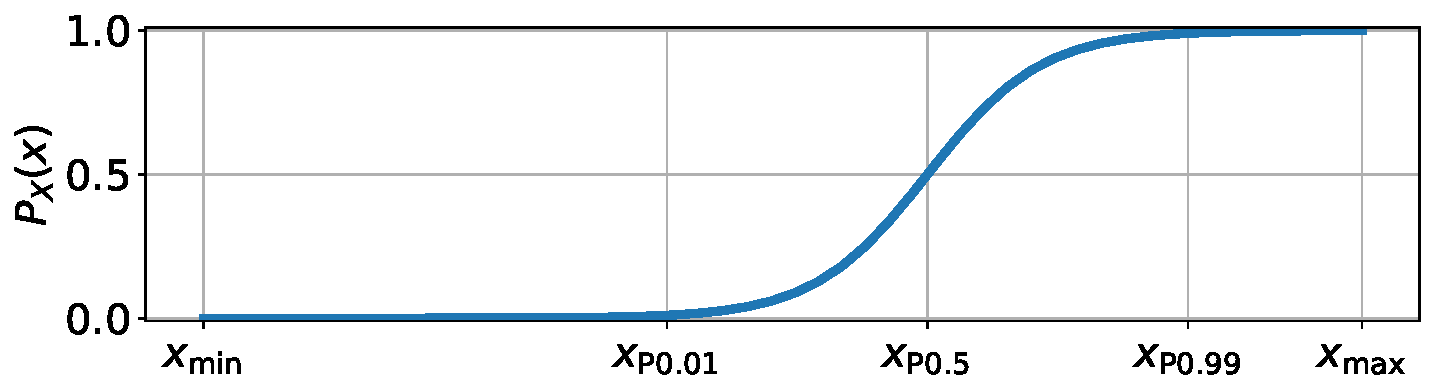
\includegraphics[width=\textwidth]{images/general_logF.pdf}
	\caption{General shape of the logistic function $P_{\rm X}(c)$ for a penalty for moving to a certain cell $c$ in the category $X$ ($\in\{\text{W, G, D, T, F}\}$). The penalty depends on a characteristic variable $x$, in combination with the thresholds, $x_{\rm P0.01}$ and $x_{\rm P0.99}$ (and $x_{\rm min}$ and $x_{\rm max}$) and, thus, the steepness parameter $k_{\rm x}$.}
	\label{fig:logF}
\end{figure}
For each category $X$, this logistic function has the same (relative) shape between $x_{\rm P0.01}$ and $x_{\rm P0.99}$ given by $k$. 
Hence, by choosing $x_{\rm P0.01}$ and $x_{\rm P0.99}$, the sensitivity of penalty $P_X$ to differences in variable $x$ is chosen. 
If $x_{\rm P0.01}$ and $x_{\rm P0.99}$ are close together, the function converges to a sigmoid function. 
If they are far apart, the function resembles a more linear increase of penalty $P_X$ with $x$.
For $x=\frac{x_{\rm P0.01} + x_{\rm P0.99}}{2}$ the penalty is $P_X = 50\%$.
Note, that if $x$ is chosen such that large values are favourable (e.g.\ for the tree and agriculture penalty), choosing values $x_{\rm P0.01}>x_{\rm P0.99}$ simply mirrors the logistic function in equation \ref{eq:P_X(c)} at $x=\frac{x_{\rm P0.01}+x_{\rm P0.99}}{2}$ and all $<$ or $>$ signs accordingly.
This logistic dependence of penalties on a characteristic variable introduces non-linear evaluation of locations.

%The steepness $k_0$ can be chosen, such that the different cases of function $P_X(x)$ are reasonably close at the threshold values $x_{\rm P0.01/P0.99}$. 
%Here, I choose $k_0 = \left( \frac{x_{\rm P0.01}-{x_{\rm P0.99}}}{2}\right)^{-1}\cdot \log\left(\frac{0.01}{0.99}\right)$, giving $P_{\rm X(x=x_{\rm P0.01})=0.01$ and $P_{\rm X(x=x_{\rm P0.99}) = 0.99$.
%Higher $k_0$ results in a steeper increase of the penalty with $x$.
%Nevertheless, this choice for parametrising a complex decision making process as well as the values for the thresholds are very flexible. 
%Of course, we can not know how Easter Island households evaluated potential new settlement areas.
%Nevertheless, archaeological data as well as logic surely show that the island has been settled progressively, e.g.\ \citet{Bahn2017}. Hence, it can be very useful to understand what 
%However, it reflects a decision. 

% Following up: Penalty Categories and summary in sketch and table
The parametrisation of evaluating new locations is, of course, strongly simplified.
First, the decision making typically depends on more than one evaluation variable per penalty category, as assumed here.
Secondly, the functional dependency of penalty w.r.t.\ the evaluation variable in general is more complex than the simple logistic evaluation in equation~\ref{eq:P_X(c)}.
However, assuming that advantages and disadvantages of a potential location (summarised in a single variable) play a non-linear role in the agent's decision making, the use of a logistic function seems reasonable\footnote{For example an agent might assign the same penalty to two locations $100\, \text{m}$ and $500\, \text{m}$ away from a large freshwater source. 
If instead the nearest lake is too far away from the agent to rely on it for everyday use, alternative sources have to be found, regardless of whether the distance is $5$ or $10\, {\rm km}$ and therefore, the penalty is similarly high.}.
I determine the choice of the evaluation variable $x$ and thresholds $x_{\rm P0.01}$ and $x_{\rm P0.99}$ by logical reasoning and rule-of-thumb estimates where necessary.
The following paragraphs point out the motivation for the specific variables for the agent's evaluation process and the threshold choices in the standard settings of the model for each penalty category $P_{\rm X}$ ($X=\{P_{\rm X}$ ($X=\{\text{G,\, W, \, D,\, T,\, F}\}$).
Table \ref{tab:x01x09} summarises the variables and corresponding thresholds that together with equation~\ref{eq:P_X(c)} determine the penalties $P_{\rm X}$ w.r.t.\ $x$ for all categories.
%All of these contributions in a cell $c$ are then linearly combined to a total penalty for this cell $P_{tot}(c)$. 

%\begin{figure}
%	Logistic Functions
%	\label{fig:Logistic}
%\end{figure}

% TOPIC: Water Distance PEnalty
\paragraph{Water Penalty $P_{\rm W}$}
There are very limited permanent sources of freshwater on the island, making it an important factor of settlement behaviour. 
Nearly all studies point out that the lakes inside the three volcano craters (Rano Kau in the South, Rano Rarakua in the East, and Rano Aroi in the North) are a dominant factor in the population's freshwater supply.
Other potential sources include pools in lava tubes and springs in the North Coast (all mentioned in \citet{Bahn2017}), an intermittent stream from Mount Terevaka, wells and water bubbles at low tide, and sugar cane juice (all mentioned in \citep{Diamond2011}), 
Additionally, \citet{Mieth2015} emphasizes the possibility to obtain a sugary sap from cut palm tree trunks, which could have replaced the need for freshwater for a large share of the population.
However, the most reliable (and accessible) large freshwater supply are the volcano craters, which, thus, are `obvious centres for human activity' \citep{Bahn2017}.
%Topic Variable xC
Consequently, I assume that potential locations close to (large) lakes are more likely settled.
The evaluation variable $w$ is radially increasing with the distance to the nearest lake weighted by the area of it:
\begin{equation}
	w = min_{\text{lake}\in \text{[Kau, Raraku, Aroi]}} \left( \frac{||
		%\begin{pmatrix} c_x \\ c_y \end{pmatrix}  - \begin{pmatrix} \vec{lake}\\ y_i \end{pmatrix}
		 \vec{c}- \vec{lake}(t)||^2}{r_\text{lake}^2\pi} \right)
\end{equation}
%\begin{equation}
%	P_W(c) = \frac{1}{N} \cdot min_{\text{lake}\in \text{[Kau, Raraku, Aroi]}} \left( \frac{\text{dist(lake, c)}^2}{r_\text{lake}^2\pi} \right)
%\end{equation}
with $r_\text{Kau} = 506\, \rm{m}$, $r_\text{Raraku} = 170\, \rm{m}$, $r_\text{Aroi} = 75\, \rm{m}$ and $\vec{lake}$ the position of the cells corresponding to the lakes.
%Here, $dist$ is the minimum straight line distance between a lake and the cell's midpoint.
%$N$ is a normalisation factor, such that the penalty $P_{\rm W}\in[0,1]$.
The thresholds are chosen as 
\begin{equation}
w_{\rm P0.01} = \frac{(0.5\, {\rm km})^2}{r_\text{Raraku}^2\pi} \qquad
 w_{\rm P0.99}=\frac{(5\, {\rm km})^2}{r_\text{Raraku}^2\pi}
\end{equation} 
($0.5$ and $5\, {\rm km}$ distance of a lake like Rano Raraku, respectively).
Then, $P_{\rm W}(c)$ is calculated from equation \ref{eq:P_X(c)} with evaluation variable $w$, the corresponding thresholds and $k_{\rm W}$ as in equation \ref{eq:k}:
\begin{equation}
	P_{\rm W}(c) = \frac{1}{1+\exp\left( - k_{\rm W} (w(c)-\frac{w_{\rm P0.01}+w_{\rm P0.99}}{2}) \right)} \ .
\end{equation}
As described before drought periods during the Medieval Climate Anomaly and the Little Ice Age potentially lead a drying especially of Rano Raraku in the period before $1200\, {\rm A.D.}$ and between $1570-1720 \, {\rm A.D.}$ \citep{Rull2020}. 
%Hence, during drought periods the locations around Rano Raraku have a substantially higher water penalty $P_{\rm W}$.
%The penalty is cut-off at its maximum value $1$, even for this case with higher penalties.
Except for these droughts, the water penalty is constant for all agents and times.
A map of $P_{\rm W}(c)$ (without drought) is shown in Figure \ref{fig:plotpw}. 
\begin{figure}
	\centering
	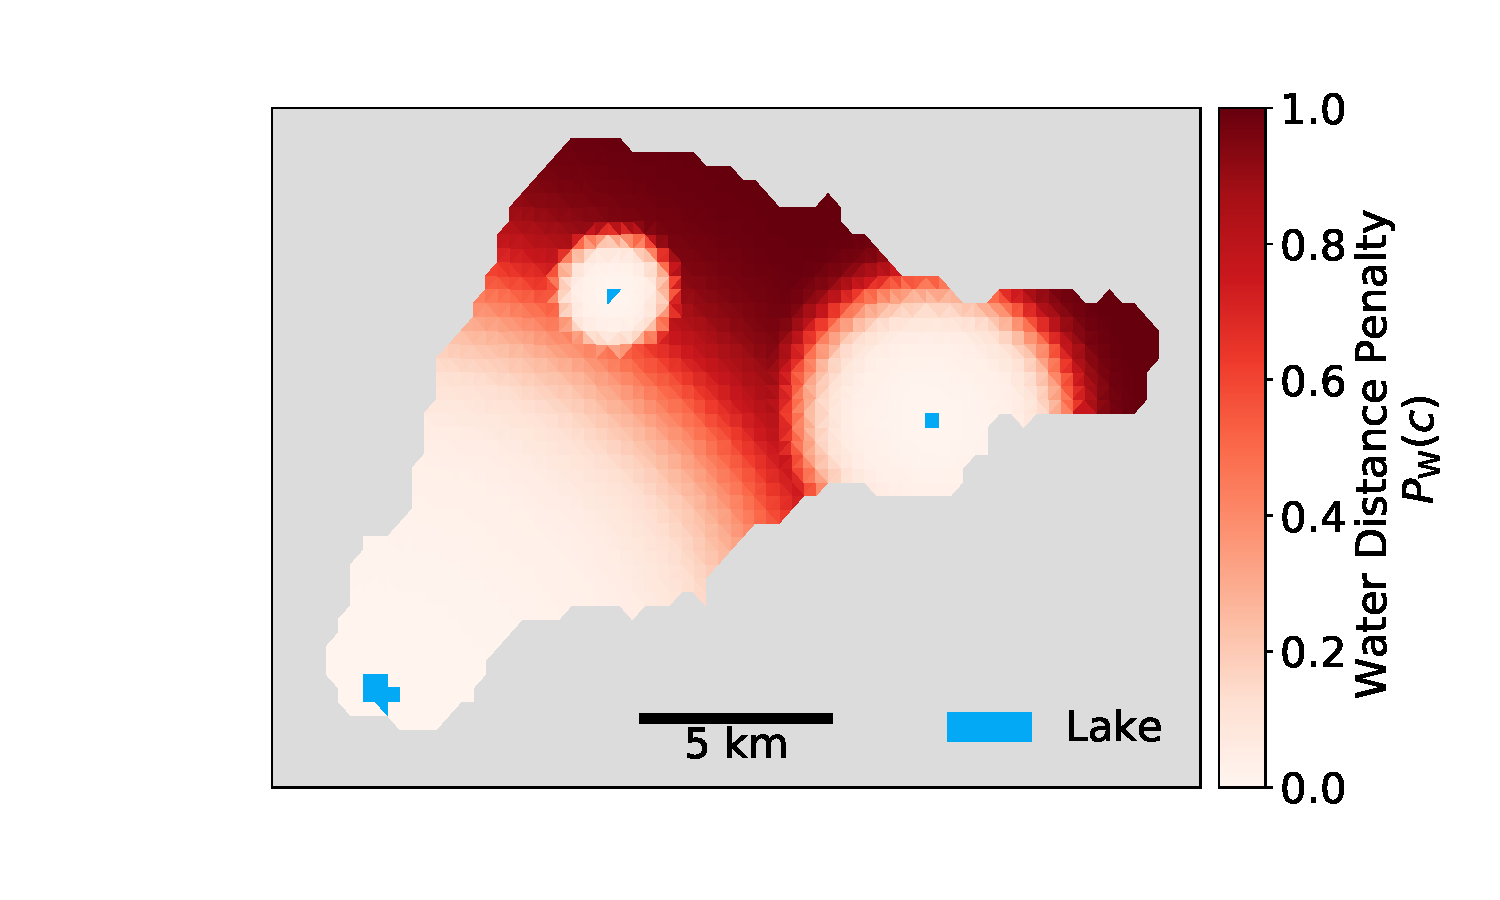
\includegraphics[width=1\linewidth]{images/Plot_PW}
	\caption{The water penalty $P_{\rm W}(c)$ for all cells in times without drought, i.e.\ in which Rano Raraku (in the East) provides freshwater.}
	\label{fig:plotpw}
\end{figure}


%Topic: Elevation Slope
\paragraph{Geographical Constraints (terrain elevation and slope) $P_{\rm G}$}
High elevation and slope of Easter Island further penalise the settlement probabilities in this model.
Archaeological evidence (e.g.\ the distribution of the Ahu and Moai) shows that the main settlements remained dominantly within the first $1-2\, \rm{km}$ of the coast, even if upland locations were farmed \citep{Bahn2017}.
There are several possible reasons for that including easier access to small-scale fishing, climatic conditions, or cultural reasons.
Hence, I assume that the geographical penalty depends on the cell's elevation.
While Easter Island is generally quite shallow, especially the North West coast and the areas around the volcano craters are steep, making it difficult for large households to settle in these spots, e.g.\ due to the danger of soil erosion. 
Hence, locations with a large slope are also penalised.
The location evaluation variables, $el(c)$ and $sl(c)$, and the corresponding chosen thresholds $el_{\rm P0.01}=min_{\rm c}(el(c))=0\, {\rm m}$ and $el_{\rm P0.99}=max_{\rm c}(el(c)) = 300\, {\rm m}$ (without any reference) for the elevation and $sl_{\rm P0.01}=0^\circ$ and $sl_{\rm P0.99}=7.5^\circ$ (without any reference) for the slope. 
Then, with corresponding $k_{\rm el}$ and $k_{\rm sl}$ from equation~\ref{eq:k}, the penalties for terrain elevation and slope are calculated as 
\begin{eqnarray}
	P_{\text{el}}(c) = \frac{1}{1+\exp\left( - k_{\rm el} (el(c)-\frac{el_{\rm P0.01}+el_{\rm P0.99}}{2}) \right)}\\
	P_{\text{sl}}(c) = \frac{1}{1+\exp\left( - k_{\rm sl} (sl(c)-\frac{sl_{\rm P0.01}+sl_{\rm P0.99}}{2}) \right)}
\end{eqnarray}
The (combined) geographical penalty $P_{\rm G}$ for a cell $c$ is simply the average of $P_{\rm el}$ and $P_{\rm sl}$:
\begin{equation}
%P_{\rm G}(c) = \rm{max}\left(P_\text{el}(c), P_\text{sl}(c) \right)
P_{\rm G}(c) = \left(P_\text{el}(c)+P_\text{sl}(c) \right)/2
\end{equation}
Figure \ref{fig:P_G} shows the geographic penalty, $P_{\rm G}$, which is constant for all agents and times.
\begin{figure}
	\centering
	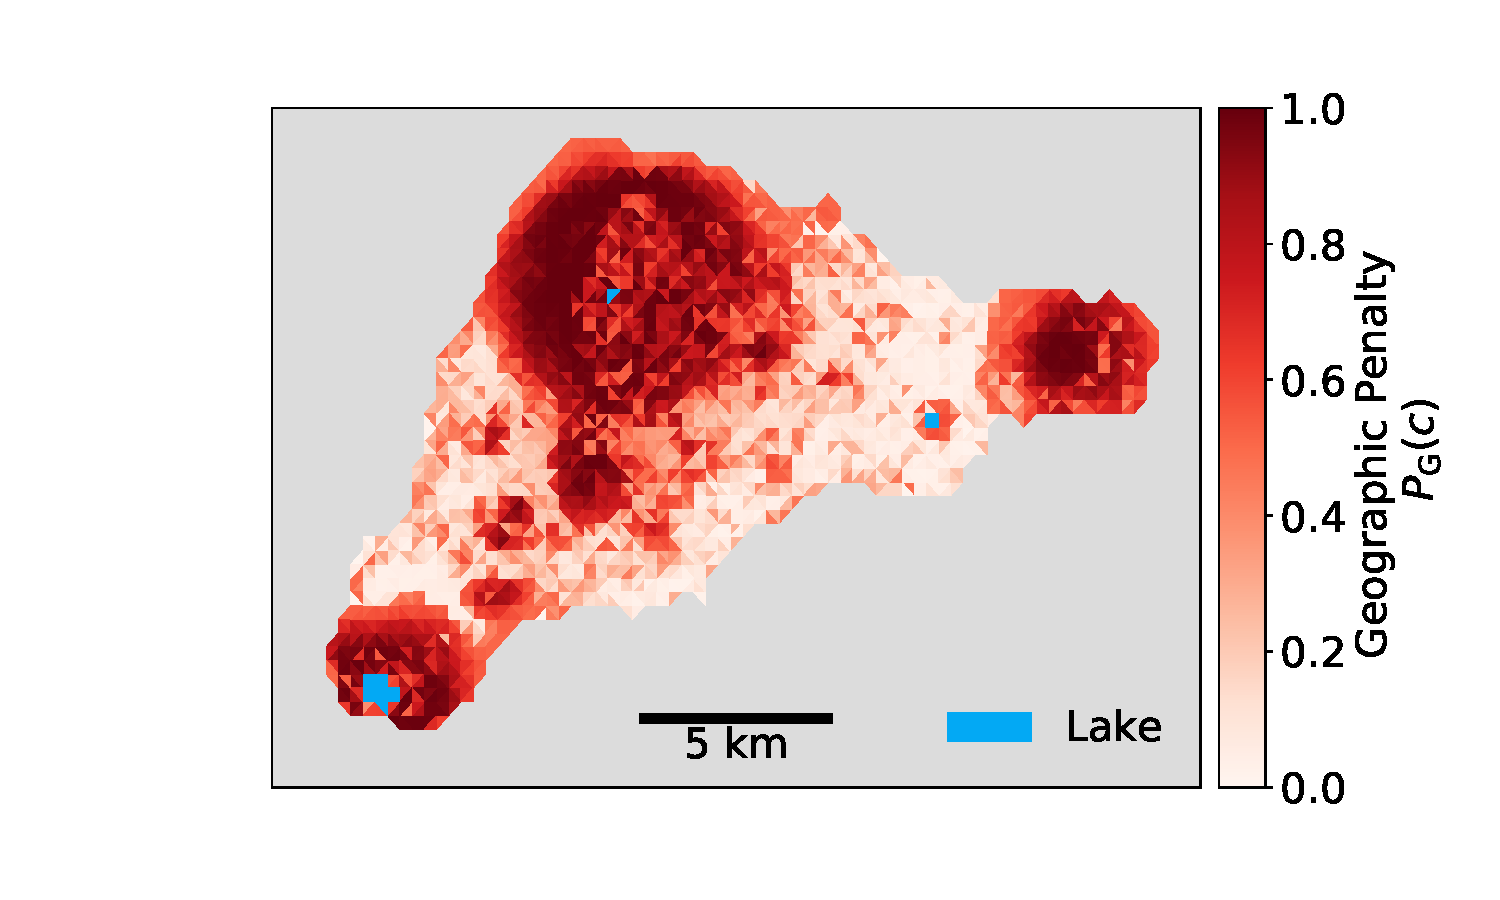
\includegraphics[width=1\linewidth]{images/Plot_PG}
	\caption{The constant geography penalty $P_{\rm G}$ for all cells.}
	\label{fig:P_G}
\end{figure}

% TOPIC: Pop Density Penalty
\paragraph{Population density $P_{\rm D}$}
Agents also avoid moving to locations with a large population density.
While different agents share the same resources and, thus, interact with the same environment, their actions and moving decisions are independent from each other. 
However, penalising potential new locations due to high population densities introduces a direct agent-agent interaction. 
To some degree, this is incorporated in the farming penalty as well, as regions with large population density, also have fewer available agriculture sites.
I define the population density of a cell as the population size in all cells within the farming radius of cell $\tilde{c}$, i.e.\ $C_{\rm F}(\tilde{c})$ divided by the corresponding area.
\begin{equation}
pd (\tilde{c}) = \frac{\mathbf{pop}|_{\hat{c} \in C_{\rm F}(\tilde{c}) }}{r_{\rm F}^2 \pi}
\end{equation}
The thresholds are chosen as
\begin{equation}
pd_{\rm P0.01} = 0 \, {\rm \frac{ppl}{km^2}}
\end{equation}
and 
\begin{equation}
pd_{\rm P0.99} = 300 \, {\rm \frac{ppl}{km^2}}
\end{equation}
with \citet{Kirch2010} estimating values of $262$ and $389\, {\rm \frac{ppl}{km^2}}$ (according to \citet{Puleston2017})on `prime agricultural land' in Hawaii and Maui, which are likely overestimates of the maximum local densities on Easter Island \citep{Puleston2017}. %Puleston state that!!
%The latter is chosen from local population density estimates of \todo{Puleston 558}.
The (time dependent) population density penalty for one cell is then
\begin{equation}
P_{\rm D}(\tilde{c}) = \frac{1}{1+\exp\left( - k_{\rm D} (pd(\tilde{c})-\frac{pd_{\rm P0.01} + pd_{\rm P0.99}}{2}) \right)}
\end{equation}
with the corresponding $k_{\rm D}$ from equation~\ref{eq:k}.
		
% TOPIC: Tree Penalty
\paragraph{Tree Availability $P_\text{T}$}
Next, scarcity of trees in the surrounding of a specific location also decreases the probability to settle there.
Hence, the tree penalty $P_{\rm T}(\tilde{c})$ is determined via the evaluation variable $tr(c)$, the number of trees within $C_{\rm T}(\tilde{c}$,
\begin{equation}
	tr(\hat{c}) = \sum_{\hat{c} \in C_{\rm T}(\tilde{c})}\, T(\tilde{c},t) \ .
\end{equation}
A cell with large value of $tr$ is assigned a lower penalty.
The threshold for negligible tree penalty, $tr_{\rm P0.01}$, is quite arbitrary.
Here, I choose that an agent considers tree availability as `optimal' if the tree number is sufficient to fill the tree requirement for a population at a very high population density of $pd = pd_{\rm P0.99}$ in the tree search radius, $C_{\rm T}(c_{\rm i}(t))$, with maximum tree preference $T_\text{Pref, max}$  for roughly one generation ($\sim 45\, {\rm yrs}$).
%a household with population size $42$ (the mean splitting population threshold) and maximum tree preference $T_\text{Pref, max}$ to fill its tree needs for the average lifespan of an individual ($\sim 45\, {\rm yrs}$)
\begin{equation}
tr_{\rm P0.01} = T_\text{Pref, max} \cdot T_\text{Requ, pP} \cdot pd_{\rm P0.99} \cdot \frac{r_{\rm T}^2}{r_{\rm F}^{2}} \, {\rm ppl} \cdot 45\, {\rm yrs} = 
216\cdot 10^3 \, {\rm trees} \ .
\end{equation} 
The value of $tr$ assigned to $99\%$ penalty is the tree number required to keep the current agent's population at a happiness level of at least $h_{\rm i}(t) = H_{equ}$ for the next year:
% $T_\text{Requ, i}(t) \cdot H_\text{equ} \cdot 5\, {\rm yrs} $
\begin{equation}% $T_\text{Requ, i}(t) \cdot H_\text{equ} \cdot 5\, {\rm yrs} $
tr_{\rm P0.99, i}= T_\text{Pref, i}(t) \cdot T_\text{Req, pP} \cdot pop_{\rm i}(t) \cdot H_\text{equ} \ ,
\end{equation}
which is typically $5-100\, {\rm trees}$ depending on the agent $i$ and the time.
On top of the logistic penalty dependency, I further enforce this limit, $tr_{\rm P0.99}$, as a necessary condition for an agent to settle in the cell $\tilde{c}$ (even if all other penalties are extremely favourable): $tr(\tilde{c}) \stackrel{!}{>} tr_{\rm P0.99}$. 
%in to relocate to a specific cell is set in place (for trees and later also farming):
%To move to a spot in cell $\tilde{c}$, 
%At least sufficient trees to reach $h_{\rm i}(t)\geq H_{\rm equ}$ in the next year have to be present, i.e.\ $tr(\tilde{c}) \stackrel{!}{>} tr_{\rm P0.99}$. Otherwise, penalty is $P_{\rm T}= \infty$ to ensure that the cell is avoided by the agent even if all other penalty contributions are favourable.
In total, 
\begin{equation}
P_{\rm T}(\tilde{c}) = 
\begin{cases} \infty & { if }tr(\tilde{c})< tr_{\rm P0.99} \\
\frac{1}{1+\exp\left( - k_{\rm tr} (tr(\tilde{c})-\frac{tr_{\rm P0.01}+tr_{\rm P0.99}}{2}) \right)} & \text{ else }
\end{cases}
\end{equation}
%Hence, agents favour locations with a large tree density around the cell.


%Unless the agent's population size is reduced or its tree preference changes the agent will have to move in the next year again though. 

%The tree penalty $P_T$ is large if the number of trees in $C_T(\tilde{c})$ around the new location $\tilde{c}$ is much smaller than its maximum on the island:
%\begin{equation}
%	T_\text{reachable}(\tilde{c}) = \sum_{\hat{c} \in C_T(\tilde{c})} \, T(\hat{c}, t)
%\end{equation}
%Again, the scaled $tanh$ function (equation \ref{eq:scaledtanh}) is used relative to the maximum number of possible trees 
%\begin{equation}
%	T_\text{max, reachables} 
%\end{equation}
%of the local number of trees in $C_T(\tilde{c})$ around the new location $\tilde{c}$ is used to derive the tree penalties:
%\begin{equation}
%	P_T = \text{scaledTanh}_T(c,T_\text{50\%P}), T_\text{100\%P}, \kappa)
%\end{equation}
%where the tree 



% TOPIC: Agric Penalty
\paragraph{Farming Land Availability $P_{\rm F}$}
%Location penalised by agriculture
Finally, availability of farming sites influences the agent's moving decision.
The penalty for farming, here, depends on two evaluation variables: 
The total available farming potential $F_\text{tot}(\tilde{c})$ and the available farming potential from non-eroded, well-suited cells only, $F_\text{well}(\tilde{c})$.
The penalties for both variables are calculated and then averaged.
The total available farming potential is simply a summation of all productivity indices of arable, unoccupied sites (i.e.\ acres within a cell) within $C_\text{F}(\tilde{c})$.
\begin{equation}
	F_\text{tot}(\tilde{c}) = \left( \sum_{\hat{c} \in C_{\rm F}(\tilde{c}) }\, F_{\rm PI}(\hat{c}) \cdot (A_{\rm acres}(\hat{c})  - \mathbf{A}_{\rm F}(\hat{c}, t) )\right) \ ,
\end{equation}
where $A_{\rm acres}(c)$ is the number of acres and $ \mathbf{A}_{\rm F}(c,t)$ is again the number of occupied sites (and, therefore, unavailable to new agents) in cell $c$ 
Similarly, the farming potential for well-suited cells only is 
\begin{equation}
	F_\text{well}(\tilde{c}) = \left( \sum_{\hat{c} \in C_{\rm F}(\tilde{c}) \ \cup \ F_{\rm PI}(\hat{c})=1} \, F_{\rm PI}(\hat{c}) \cdot (A_{\rm acres}(\hat{c})  - \mathbf{A}_{\rm F}(\hat{c},t) )\right) \ .
\end{equation}
This $F_\text{well}$ is an important consideration for agents as it makes cells more favourable, if the farming produce can be obtained from a few well-suited rather than a larger number of poorly suited sites, with a larger number of workers involved.

The threshold for an optimal location w.r.t.\ farming is the maximum possible land needed to be farmed by an agent with population $42$.
\begin{eqnarray}
F_\text{well, P0.01} & = & F_\text{tot, P0.01} =  (1-T_\text{pref, min})\cdot F_\text{Req, pP} \cdot 42\, {\rm ppl}  \\
& = & 
\begin{cases} 16.8\, {\rm acres}  \text{ (with }F_{\rm PI}(c)=1\text{) for high N fixation scenario} \\  57.1 \, {\rm acres} \text{ (with }F_{\rm PI}(c)=1\text{) for low N fixation scenario} \nonumber
\end{cases} 
\end{eqnarray}
The threshold for penalty $P_{\rm F}(c)=0.99$ is the agent's current farming requirement sufficient to obtain happiness $h_{\rm i}(t) = H_{\rm equ}$, i.e.\
\begin{equation} 
F_\text{well, P0.99, i} = F_\text{tot, P0.99} = (1-T_\text{pref, i}(t))\cdot F_\text{Req, pP}\cdot pop_{\rm i}(t) \cdot H_{equ}
\end{equation}
depending strongly on the tree preference and population.
The parameter, $k_{\rm F}$ is the same for both evaluation variables $F_\text{well} $ and $F_\text{tot}$.

As for trees, a necessary condition for moving to a cell is enforced:
 If the total\footnote{And, hence, also the well-suited} farming potential $F_\text{tot}(\tilde{c})$ at a cell $\tilde{c}$ is smaller than $F_\text{tot, P0.99}$, the farming penalty is set to $P_{\rm F}(\tilde{c}) = \infty$ (and thus the cell is not considered regardless of other penalties).
 % , for all cells with $Y_\text{tot}(\tilde{c})< A_\text{Req, i}(t) \cdot H_{equ}$ (i.e.\ $a_\text{tot} < a_\text{tot, P0.99}$), the penalty is set to $P_F(\tilde{c})=1$ 
Then, the total penalty is 
\begin{equation}
P_{\rm F} (\tilde{c}) = 
\begin{cases} 
\infty & \text{ if } F_\text{tot} < F_\text{tot, P0.99}\\
\frac{0.5}{1+\exp\left( - k_{\rm F} (F_\text{well}(c)-F_\text{P0.5}) \right)} + \frac{0.5}{1+\exp\left( - k_{\rm F} (F_\text{tot}(c)-F_\text{P0.5}) \right)} & \text{ else}
\end{cases}
\end{equation}
with $F_\text{P0.5} = \frac{F_{\rm P0.01}+F_{\rm P0.99}}{2}$.
In summary, the farming penalty is smallest for those cells surrounded by a lot of well-suited, available sites.
The penalty is large for those cells surrounded by few available, arable sites in general and few available, well-suited sites in cells in particular.
%E.g.\ penalty $P_{\rm F}=0.5$ 

In locations around Anakena Beach, where open-sea fishing is allowed, the agents do not farm. 
The farming penalty in theses cells should not depend on availability arable land and instead encourage agents to move to this location.
Hence, I decide to set the `farming' penalty in these cells to
\begin{equation}
	P_{\rm F}(\hat{c}) = - 1 %(1-T_\text{Pref, i}(t)) 
	 \quad \forall \  \hat{c} \in C_\text{F}(c_{\rm Anakena})
\end{equation}


 \begin{table}
	\centering
	\begin{tabular}{c|c|K|c|c|L}
		$X$ & $x$& Description & $x_{\rm P0.01}$ & $x_{\rm P0.99}$ & Necessary Condition \\ \hline
		W &$w$ & Area weighted distance of cell to lake & $\frac{(0.5\, {\rm km})^2}{r_\text{Raraku}^2\pi}$ & $\frac{(5\, {\rm km})^2}{r_\text{Raraku}^2\pi}$\\
		G & & & & & \\
		& $el$ & Elevation & $0\, {\rm m}$ & $300\, {\rm m}$ & \\
		& $sl$ & Slope & $0^\circ$ & $7.5^\circ$ & \\
		D & $pd$ & Population density within $r_{\rm F}$ & 0 & $300\, {\rm \frac{ppl}{km^2}}$ & \\
		T & $tr$ & Number of trees within $r_{\rm T}$ & $216\cdot 10^3$ & $\sim 5-100^* \, {\rm Trees}$ &  at $x_{\rm P0.99}$\\
		F & & & & & \\
		& $F_{\rm tot}$ & Total possible farming produce within $r_{\rm F}$ & $16.8 \, \rm{acres}$  & $\sim 1-13^* \, \rm{acres}$& at $x_{\rm P0.99}$\\
		& $F_{\rm well}$ & Possible farming produce of well-suited sites within $r_{\rm F}$ & -"- & -"- & -"-\\
	\end{tabular}
\caption{The evaluation variable and chosen thresholds for each penalty category.
	Inserting these into the logistic function (equation~\ref{eq:P_X(c)}) gives the penalties in each category:
	$P_{\rm G}$ for geography, $P_{\rm W}$ for freshwater proximity, $P_{\rm D}$ for population density, $P_{\rm T}$ for tree availability, $P_{\rm F}$ for farming land availability.
	Note, that $x_{\rm P0.99}$ for category $T$ and $F$, representing the minimum amount of resources required, depend on the specific agent's properties (denoted by $^*$).
	This value is a further minimum condition for moving to the cell. For the farming penalty, the thresholds are calculated for the high Nitrogen fixation scenario here.
	For $P_{\rm G}$ and $P_{\rm F}$, which have two elevation variables, the mean of the sub penalties gives the corresponding category penalty.
}
\label{tab:x01x09} 
\end{table}


\paragraph{From Penalties to Probability}
% TOPIC: From Penalty to Pop, and mask, no sites left?
The resulting penalties for a cell  $\tilde{c}$ in $C_{\rm M}(c_{\rm i}(t))$ from all categories are linearly combined to obtain a total penalty, which is then converted to a discrete probability $Pr(\tilde{c})$ of moving to this cell.
With (normed) weights $\vec{\alpha}$ (and the agent's tree preference $T_\text{Pref, i}(t)$):
\begin{equation}\label{eq:vecalpha}
\vec{\alpha} = \left(\alpha_{\rm G},  \alpha_{\rm W}, \alpha_{\rm D},  \frac{T_\text{Pref, i}(t)}{\eta_{\rm i}(t)} \cdot \alpha_{\rm T}, \frac{(1-T_\text{Pref, i}(t))}{\eta_{\rm i}(t)} \alpha_{\rm F}\right)
\end{equation} 
where $\eta_{\rm i}(t) = \frac{\alpha_{\rm T} T_\text{Pref, i}+ \alpha_{\rm F} (1-T_\text{Pref, i})}{\alpha_{\rm T}+\alpha_{\rm F}}$ is a normalisation factor to ensure that, $\frac{T_\text{Pref, i}(t)}{\eta_{\rm i}(t)}\cdot \alpha_{\rm T} + \frac{(1-T_\text{Pref, i}(t))}{\eta_{\rm i}(t)} \cdot \alpha_{\rm F} = \alpha_{\rm T}+ \alpha_{\rm F}$ and, therefore, $||\vec{\alpha}||=1$. 
The total penalty is:
\begin{equation}
P_\text{tot, i}(t) =  \begin{cases} \infty & \text{ if } \tilde{c}\notin C_{\rm M}(c_{\rm i}(t))\\
	 \langle \vec{\alpha}{, } \vec{P} \rangle &  \text{ else}
	 \end{cases}
\end{equation}
with $\vec{P} = (P_{\rm G}, P_{\rm W}, P_{\rm D}, P_{\rm T}, P_{\rm F})$.
Finally, 
\begin{equation}
	Pr(\tilde{c})  = \frac{1}{N} \cdot \exp \left( - \gamma \cdot P_{tot}(c) \right) 
\end{equation}
where $N$ is a normalisation and $\gamma$ is a dimensionless scaling factor, which represents the agent's tendency to actually follow the penalty evaluation. 
By increasing $\gamma$, the agent's move less likely to spaces with low probability (high total penalty). 
E.g.\ for $\gamma$ \ra $\infty$, agents have perfect knowledge of the island's properties and move to the optimal cell with minimal penalty, i.e.\ the decision making is an increasingly deterministic optimisation process\footnotemark.
\footnotetext{Proof: Let's consider the relation between $Pr(c_\text{min})$, where $c_\text{min}$ denotes the cell with the minimal penalty, and $Pr(c)$ for all cells $c$. Then, $Pr(c_\text{min})/Pr(c) = \exp(-\kappa P_\text{tot, min})/ \exp(-\kappa P_\text{tot}(c)) = \exp(-\kappa(P_\text{tot, min}-P_\text{tot}(c)))$. For $\gamma$ \ra $\infty$ this is $\delta_{c=c_\text{min}}$.}
On the other hand, $\gamma=0$ implies that agent's just move to a any new location without consideration of the penalties associated with this new location.
By choosing $\gamma$ large, but finite, I set the agents up to make individualistic, semi-rationale choices when moving, but include stochasticity (e.g.\ due to imperfect knowledge) in the decision.
An agent moves to a site based on individual assessment.
However, multiple agents share the same local environment and, thus, can quickly change the conditions of a location (e.g.\ by deforesting). 
Hence, when agents in this model decide on relocating their settlement, they do not calculate the society's optimal outcome as often assumed in mathematical models (\citet{Good2006} or \citet{Bookstaber2019}).
They decide by avoiding locations that currently seem unfavourable based on their knowledge of the current situation.
% choosing a well suited location to surviving and increasing their population size.

Having selected a new cell, the agent chooses a location within this cell with uniform probability.
Note, that the actual availability of arable, free land and/or trees, might deviate slightly from the calculation of the cell's penalty (and corresponding probability), as the location of the settlement differs from the cell's midpoint, which was used for the penalty evaluation.
This accuracy error decreases with higher discretisation resolution.
The total procedure of calculating the probability is sketched in Figure \ref{fig:sketchmoving}.

\begin{figure}
	\centering
	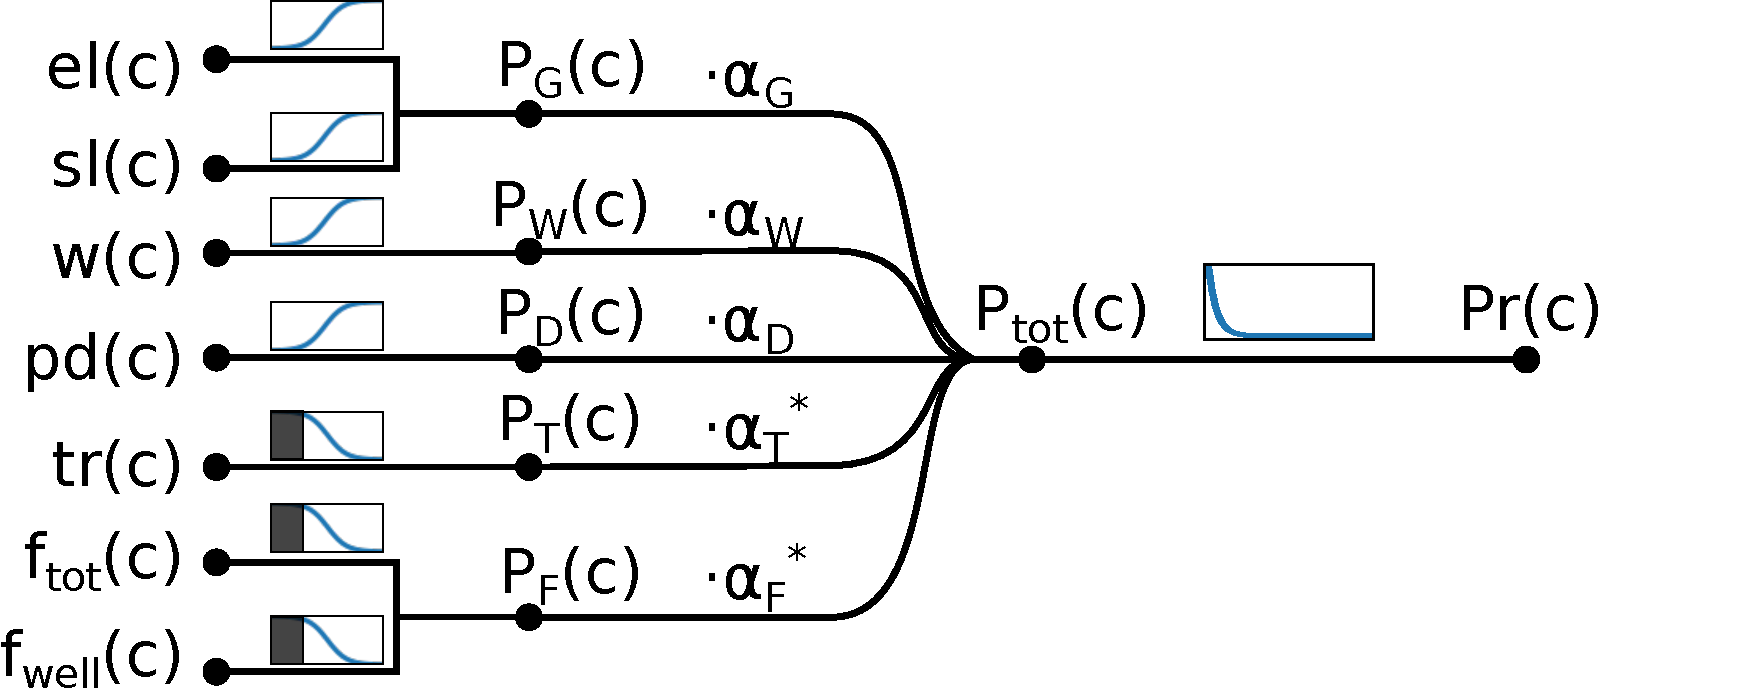
\includegraphics[width=1\textwidth]{images/SketchABM2/sketchMoving}
	\caption{A sketch of the calculation of the probability for agent $i$ to relocate its settlement to cell $c$: The category penalties ($P_{\rm G}$ for geography, $P_{\rm W}$ for freshwater proximity, $P_{\rm D}$ for population density, $P_{\rm T}$ for tree availability, $P_{\rm F}$ for farming land availability) are calculated via one or two characteristic evaluation variables described in the main text assuming a logistic functional dependence (blue curves). 
	If two evaluation criteria are considered for one category, the resulting sub-penalties are averaged (crossings for $P_{\rm G}$ and $P_{\rm F}$).
	For $P_{\rm T}$ and $P_{\rm F}$, cells that do not have the minimum required resource availability are excluded (black boxes).
	The total penalty for cell $c$, $P_{\rm tot}(c)$ is then a linear superposition of all category penalties (with the weights $\alpha_{\rm T}^*$ and $\alpha_{\rm F}^*$ adjusted according to the tree preference $T_{\rm Pref, i}(t)$ (equation \ref{eq:vecalpha}).
	The final probability for a cell $c$ is derived as $Pr(c) \sim e^{-\gamma \cdot P_{\rm tot}(c)}$ (blue line in the right part), with scaling factor $\gamma$.} 
	\label{fig:sketchmoving}
\end{figure}



% TOPIC: When does it occur, calc penalty in each day, \ldots
With this procedure, agent's move (as resource availability becomes scarce or a subgroup splits from a large household) according to environmental features. 
The specific settings create spatial patterns of settlement behaviour which in turn non-linearly change the agent-environment interaction and, thus, environment dynamics overall.

This evaluation of potential sites when an agent moves is the bottleneck w.r.t.\ computation time in this model.
The process scales quartic with the grid resolution $\delta_{\rm x,y}$, i.e.\ $\mathcal{O}(\delta_{\rm x,y}^4)$, the number of grid points per unit of length: The overall Number of cells $N_{\rm c}$ increases quadratic with $\delta_{\rm x,y}$ and the evaluation of penalties (e.g.\ summing up trees from cells in $C_{\rm T}(\tilde{c})$) for a single cell also scales quadratic with the grid resolution.
In order to increase efficiency, I use dot products and distance matrix computation from the python packages `numpy' \citep{numpy} and `scipy' \citep{scipy}, both implemented in \CC.
An alternative implementation might adjust penalties immediately when the agent's interact with the environment, which would scale as $\mathcal{O}(\delta^2\cdot N_{\rm agents}(t)\cdot N_{\rm timesteps})$.
However, since the resolution does not have to be too small for this study, and the number of moving actions is usually small compared to $N_{\rm c}$ and $N_{\rm timesteps}$, the first implementation is still reasonably fast.
	
		
% Measure Agric Productivity in acres of high quality sites
% Why Wood is a primary resource
% Tree Pref changes quickly
% Mention non-reneqabl etc. earlier.
% Burning not really sure??
% Define SItes(c) as int(area)
% mention arable very early and farmed land
		
\section{Standard Run and Sensitivity Analysis}
The resulting model has a multitude of parameters, settings and parametrisations often associated with large uncertainties. 
There are in principle two different kinds of parameter choices described in the following paragraphs and summarised in Table \ref{tab:sensitivity}.

\begin{table}
	\begin{tabular}{l|K|H}
%		Parameter &  Std Run & Fix? & Sensitivity Analysis \\ \hline
%		$t_{\rm arrival}$ & $800\, {\rm A.D.}$ & fix & Mostly only important for timing \\
%		$\mathbf{pop}_{\rm arrival}$ & $40$ & fix & -"- (within reasonable estimates)\\ \hline
%		 $F_\text{ Req, pP}$ & $0.5\, {\rm \frac{acres}{person}}$ & 2 & two different environmental scenarios \citep{Puleston2017}\\
%		 $F_\text{PI, [well, eroded, poor]}$ & $[0.8,\ 0.5,\ 0.1]$ & fix & strong impact (especially poor vs.\ well), estimated from \citet{Louwagie2006} \\
%		 $T_\text{Req, pP}$ & $5\, {\rm \frac{Trees}{person\cdot yr}}$ & 2 & strong impact 
%		 estimate from \citet{Brandt2015}, tested 

		Parameter &  Std Run & Sensitivity Tests \\ \hline
		$t_{\rm arrival}$ & $800\, {\rm A.D.}$ & --\\
		$\mathbf{pop}_{\rm arrival}$ & $40$ & --\\ \hline
		 $F_\text{ Req, pP}$ & $0.5\, {\rm \frac{acres}{person}}$ &  $1.7\, {\rm \frac{acres}{person}}$ \\
		 $F_\text{PI, [well, eroded, poor]}$ & $[0.8,\ 0.5,\ 0.1]$ & -- \\
		 $T_\text{Req, pP}$ & $5\, {\rm \frac{Trees}{person\cdot yr}}$ & $10\, {\rm \frac{Trees}{person\cdot yr}}$  \\
		  $T_\text{Pref, min}$ & $0.2$ & -- \\
		  $T_\text{Pref, max}$ & $0.8$ & --\\
		  $T_\text{Pref, min}|_{\rm fisher}$ & $0.5$ & --\\
		  $N_\text{Fisher, Max}$ & $10$ & -- \\ \hline
		  $\mathbf{T}(t_\text{arrival})$ & $16\cdot10^6$ & -- \\
		  $g_{\rm T}$ & $0$ & $5\%/{\rm yr}$ (with tree pop up of $0.5\%/{\rm yr}$ of carrying capacity on barren land for $10\, {\rm yrs}$) \\
		  \hline
		  $g(H_{\rm i}(t))$ (scale) & $0.1$ & --\\
		  $g(H_{\rm i}(t))$ (shape) & $1.95$ & $3$ \\
		  $g(H_{\rm i}(t)=1)$ & $1.007$ & -- \\ \hline \hline
		   Tree Pattern & uniform density for $el(c)<450{\rm m}$, $sl(c)<10^\circ$ & -- \\ \hline
		  $pop_{\rm min}$ & 6 & --\\
		  $pop_\text{max, mean}$ & 42 & --\\
		  $pop_\text{max, std}$ & 3 & -- \\
		  $pop_{\rm split}$ & 12 & --\\ \hline
		  $r_{\rm F}$ & $1\, {\rm km}$ & --? \TODO\\
		  $r_{\rm T}$ & $2\, {\rm km}$ & --? \TODO \\ \hline 
		  $f_{\rm Tree\  Pref}$ & linear & delayed, careful, logistic\\ \hline 
		  $r_{\rm M}$ & $5\, {\rm km}$ (if $\mathbf{pop}(t)>5000$) & --? \TODO \\
		  $x_{\rm P0.01}$ & Table \ref{tab:x01x09} & -- \\
		  $x_{\rm P0.99}$ & Table \ref{tab:x01x09} & -- \\
		  $\vec{\alpha}$ & $(0.2,0.2,0.2,0.2,0.2)$ & $(0.0,0.0,0.0,0.5,0.5)$\\
		  $\gamma$ & $20$ & $0$, $100$ \TODO \\
		  Droughts & $800-1200$, $1570-1720$ & -- \\
	\end{tabular}
	\caption{Choices of parameters for the standard run and sensitivity analysis. The upper half (separated by double line) mainly determines the aggregated population dynamics, the lower half determines the microscopic behaviour and thus influences mainly the spatial patterns.}
	\label{tab:sensitivity}
\end{table}

The first category of parameters influences directly the island wide, aggregate population dynamics and peak population because they determine the amount of resource acquisition and availability per agent and the population growth with respect to harvest success (or agent's happiness): 
\begin{itemize}
	\item the resource requirements calculated from the constant farming requirement per person $F_\text{ Req, pP}$ in combination with the farming productivity indices $F_\text{PI, [well, eroded, poor]}$, the tree harvest requirement per person $T_\text{Req, pP}$ as well as the values for $T_\text{Pref, min}$, and with a lower importance $T_\text{Pref, max}$, $T_\text{Pref, min}|_{\rm fisher}$ and $N_\text{Fisher, Max}$
	\item the initial number of trees $\mathbf{T}(t_\text{arrival})$ and (if regeneration is enabled) the tree regeneration parameters, i.e.\ the logistic growth rate $g_{\rm T}$, and pop up properties on barren land 
	\item the demography model parameters, i.e.\ the shape and scale of the population size growth rate function depending on the harvest success $g(H_{\rm i}(t))$ and the initial population growth rate $g(H_{\rm i}(t)=1)$.
\end{itemize}
%These parameters have a direct influence on the dynamics of the aggregated population size and its peak value.
Furthermore, the parameters $t_{\rm arrival}$ and $\mathbf{pop}_{\rm arrival}$ simply influence the timing of the dynamics.
The uncertainties associated with these parameters are the main source for the  
discrepancies between contradictory theories about the history of Easter Island.
This model presented here does not aim to dispute one theory or the other.
In fact, the model can re-create the proposed population dynamics by adjusting some of the parameters above.
Hence, while choosing a standard set of parameters, I also investigate some alternative settings of these parameters (shown in Table \ref{tab:sensitivity}) giving rise to different proposed theories of pre-history population dynamics on Easter Island.

The novel part of this study, however is the spatially explicit component and the stochastic, microscopic acting and decision making of the agents in the model.
The values of parameters associated with this second category are even less known, but as described in the Introduction, reasonable assumptions on the values and functional dependences of the parameters can be made more naturally on the microscopic than the macroscopic level. The parameters in this category are related to the
\begin{itemize}
	\item household size, i.e.\ the maximum and minimum population size  of an agent ($pop_{\rm min}$, $pop_\text{max, mean}$, $pop_\text{max, std}$, $pop_\text{split}$)
	\item resource search radii ($r_{\rm F}$, $r_{\rm T}$ (in combination with the initial spatial distribution of trees, i.e.\ $T(c,t=t_{\rm arrival})$ for cells $c$)
	\item shape of the response of the tree preference to the changing local environment
	\item decision making process when moving, i.e.\ the restricted moving radius $r_{\rm M}$, penalty categories and their logistic dependency specified by the thresholds $x_{\rm P0.01}$ and $x_{\rm P0.99}$, the weights $\vec{\alpha}$, and the scale parameter $\gamma$.
\end{itemize}

% Every Run is a realisation: 
Since multiple processes in the model are stochastic, each run is only a single realisation. 
While the aggregated results do not differ much between runs with the same setting, the spatial pattern of deforestation varies in general. 
I perform several ensemble runs, but there is no obvious way to obtain an aggregate spatial mean dynamics per se.
Instead, variation in spatial patterns for the same experiment are described qualitatively.

% Standard Run with table and then Average and Std
Throughout the thesis, I have defined parameter setting for a standard run (details in Table \ref{tab:sensitivity}).
I perform several sensitivity simulations (also described in Table \ref{tab:sensitivity}) and analyse the corresponding changes to this standard run in both categories of parameters related to the aggregate population dynamics and to the spatial patterns.
% Perform sensitivity analysis of second for different settings of first categories.

% From standard run, try different moving probabilities.

